\documentclass[]{book}
\usepackage{lmodern}
\usepackage{amssymb,amsmath}
\usepackage{ifxetex,ifluatex}
\usepackage{fixltx2e} % provides \textsubscript
\ifnum 0\ifxetex 1\fi\ifluatex 1\fi=0 % if pdftex
  \usepackage[T1]{fontenc}
  \usepackage[utf8]{inputenc}
\else % if luatex or xelatex
  \ifxetex
    \usepackage{mathspec}
  \else
    \usepackage{fontspec}
  \fi
  \defaultfontfeatures{Ligatures=TeX,Scale=MatchLowercase}
\fi
% use upquote if available, for straight quotes in verbatim environments
\IfFileExists{upquote.sty}{\usepackage{upquote}}{}
% use microtype if available
\IfFileExists{microtype.sty}{%
\usepackage{microtype}
\UseMicrotypeSet[protrusion]{basicmath} % disable protrusion for tt fonts
}{}
\usepackage[margin=1in]{geometry}
\usepackage{hyperref}
\hypersetup{unicode=true,
            pdftitle={The Book of OHDSI Korea},
            pdfauthor={OHDSI-Korea},
            pdfborder={0 0 0},
            breaklinks=true}
\urlstyle{same}  % don't use monospace font for urls
\usepackage{natbib}
\bibliographystyle{apalike}
\usepackage{longtable,booktabs}
\usepackage{graphicx,grffile}
\makeatletter
\def\maxwidth{\ifdim\Gin@nat@width>\linewidth\linewidth\else\Gin@nat@width\fi}
\def\maxheight{\ifdim\Gin@nat@height>\textheight\textheight\else\Gin@nat@height\fi}
\makeatother
% Scale images if necessary, so that they will not overflow the page
% margins by default, and it is still possible to overwrite the defaults
% using explicit options in \includegraphics[width, height, ...]{}
\setkeys{Gin}{width=\maxwidth,height=\maxheight,keepaspectratio}
\IfFileExists{parskip.sty}{%
\usepackage{parskip}
}{% else
\setlength{\parindent}{0pt}
\setlength{\parskip}{6pt plus 2pt minus 1pt}
}
\setlength{\emergencystretch}{3em}  % prevent overfull lines
\providecommand{\tightlist}{%
  \setlength{\itemsep}{0pt}\setlength{\parskip}{0pt}}
\setcounter{secnumdepth}{5}
% Redefines (sub)paragraphs to behave more like sections
\ifx\paragraph\undefined\else
\let\oldparagraph\paragraph
\renewcommand{\paragraph}[1]{\oldparagraph{#1}\mbox{}}
\fi
\ifx\subparagraph\undefined\else
\let\oldsubparagraph\subparagraph
\renewcommand{\subparagraph}[1]{\oldsubparagraph{#1}\mbox{}}
\fi

%%% Use protect on footnotes to avoid problems with footnotes in titles
\let\rmarkdownfootnote\footnote%
\def\footnote{\protect\rmarkdownfootnote}

%%% Change title format to be more compact
\usepackage{titling}

% Create subtitle command for use in maketitle
\providecommand{\subtitle}[1]{
  \posttitle{
    \begin{center}\large#1\end{center}
    }
}

\setlength{\droptitle}{-2em}

  \title{The Book of OHDSI Korea}
    \pretitle{\vspace{\droptitle}\centering\huge}
  \posttitle{\par}
    \author{OHDSI-Korea}
    \preauthor{\centering\large\emph}
  \postauthor{\par}
      \predate{\centering\large\emph}
  \postdate{\par}
    \date{2019-06-06}

\usepackage{booktabs}
\usepackage{amsthm}
\makeatletter
\def\thm@space@setup{%
  \thm@preskip=8pt plus 2pt minus 4pt
  \thm@postskip=\thm@preskip
}
\makeatother

\begin{document}
\maketitle

{
\setcounter{tocdepth}{1}
\tableofcontents
}
\hypertarget{introduction}{%
\chapter{Introduction}\label{introduction}}

최근 전세계적으로 의료 빅데이터 활용에 대한 논의가 뜨겁다.보건 빅데이터를 이용하여 질병 예방에 따른 의료비 절감, 의료기관의 운영비용 절감, 오류에 따른 손실비용 절감 등의 경제적 효과도 기대되어 활용이 증대되고 있다. 최근 헬스케어 서비스를 통해 생산되는 건강정보 관리와 활용에 대한 논의가 활발히 진행되고 있으며, 의료 빅데이터에 대한 니즈와 관련 데이터, 대응 방향 등이 이슈화되고 있다.

보건 의료 빅데이터 구축을 위해 다양한 노력이 진행되어 왔으며, 그 중 최근 부상하고 있는 분야는 공통 데이터 모델 (Common Data Model, CDM) 기반의 분산 연구망 (Distributed Research Network, DRN) 이다. 여러 가지의 CDM / DRN 모델이 있지만, 한국에서는 오몹 공통 데이터 모델 (OMOP-CDM) 기반의 오딧세이 네트워크 (OHDSI network) 가 사실상 표준으로 자리잡고 있다.

OHDSI 네트워크는 오픈 소스 연구 네트워크 (open-source research network)로써 데이터 아키텍처부터 시작하여 매우 방대한 오픈소스 프레임워크를 제공하고 있지만, 이러한 자료들이 잘 정리되어 있지 않아 많은 사람들이 어려움을 겪고 있었다.

본 도서는, 부족하지만 OHDSI 네트워크의 안내서가 되고자 한다.

\hypertarget{ohdsiCommunity}{%
\chapter{The OHDSI Community}\label{ohdsiCommunity}}

\emph{Seng Chan You}

\hypertarget{ohdsi-}{%
\section{OHDSI 홈페이지}\label{ohdsi-}}

\href{https://www.ohdsi.org/}{국제 OHDSI 네트워크 공식 홈페이지}를 참고하기 바란다. \href{https://www.ohdsi-korea.org/}{한국 OHDSI 네트워크 홈페이지}도 곧 오픈 예정이다.

\hypertarget{drnCdm}{%
\section{분산연구망과 공통데이터모델}\label{drnCdm}}

\hypertarget{distributed-research-network}{%
\subsection{분산연구망 (Distributed Research Network)}\label{distributed-research-network}}

의료 데이터는 데이터 구조, 형식의 이질성, 데이터의 질과 양 등 기술적인 어려움과 기관의 허락, 개인정보보호문제 등 법적 문제 그리고 타인에게 제공하는 데이터가 자신에게 불리하게 사용될지 모른다는 두려움 등 자신의 자료를 타인과 공유하고 싶지 않는 문제들이 있어 공유가 쉽지 않았다. 현재까지 대부분의 기관간 공동 연구는 극히 일부의 환자 데이터를 연구 주도 기관과 공유함으로써 진행하였는데, 한 번의 공동 연구를 위해 막대한 노력과 시간, 자금이 들어가는 현실적인 문제와 개인 정보의 공유라는 윤리적인 문제들이 있어 왔다.

이런 제약을 극복하는 방법 중 하나가 분산연구망이다. 이는 의료데이터 유통의 제약 요인 극복을 위해 병원과 기업 등 수요자 간에 원본데이터의 공유 없이 분산된 형태로 데이터를 관리하면서 기관 내에서 분석한 결과만 필요 할 때 거래하는 방식이다.

쉽게 설명하면, 각 병원의 환자정보를 표준화 및 익명화한 후 데이터를 병원 폐쇄망 안에 두고 사용자의 요청에 따라서 기관 안에서 분석코드/프로그램을 실행해 분석된 요약 집합정보(평균, 합, 표준편차, 오즈비, 위험도 등)만 수요자에게 회신하는 방식이라고 할 수 있다. 수요자는 폐쇄망 안에 있는 환자의 개별 정보를 보거나 취득할 수 없지만, 전체 데이터를 모아서 분석한 것과 동일한 분석 결과를 도출할 수 있다. 여러 기관에서 자료를 통합하기 위해서는 공통데이터모델이 적용되어야 한다.

\hypertarget{common-data-model}{%
\subsection{공통데이터모델 (Common Data Model)}\label{common-data-model}}

앞서 설명했듯이 데이터 표준화는 연구자들이 연구에 사용할 데이터를 공통 형식으로 저장하여 협업 연구, 대규모 분석 및 정교한 도구 및 방법론 공유를 가능하게 하는 중요한 프로세스이다. 하지만 표준화 작업을 하기 위해서는 오랜 시간과 비용이 소요된다.

이런 문제를 해결하기 위해 등장한 것이 공통데이터모델이다. 이는 여러 병원들의 데이터를 효율적으로 활용하기 위하여 정의한 표준화된 데이터 구조이다. 다기관 공동 연구 수행 시에 기관별로 서로 다른 데이터 구조로 인해 다양한 어려움이 따르는 것을 해결해 주는 방식으로 기관별로 상이한 데이터 구조와 의미를 동일한 하나의 구조와 의미를 갖도록 변환하는 벙법이라고 이해하면 쉽다.

공통데이터모델을 따르기 위해서는 각 병원이나 기관이 기존의 데이터를 공통데이터모델로 변환하는 과정이 필요하다. 이를 ETL(Extract, Transform, Load) 이라 한다. 공통데이터모델은 기존의 한계점 등을 고려하여 지속적으로 업데이트 되고 있는 중이다.

\begin{figure}
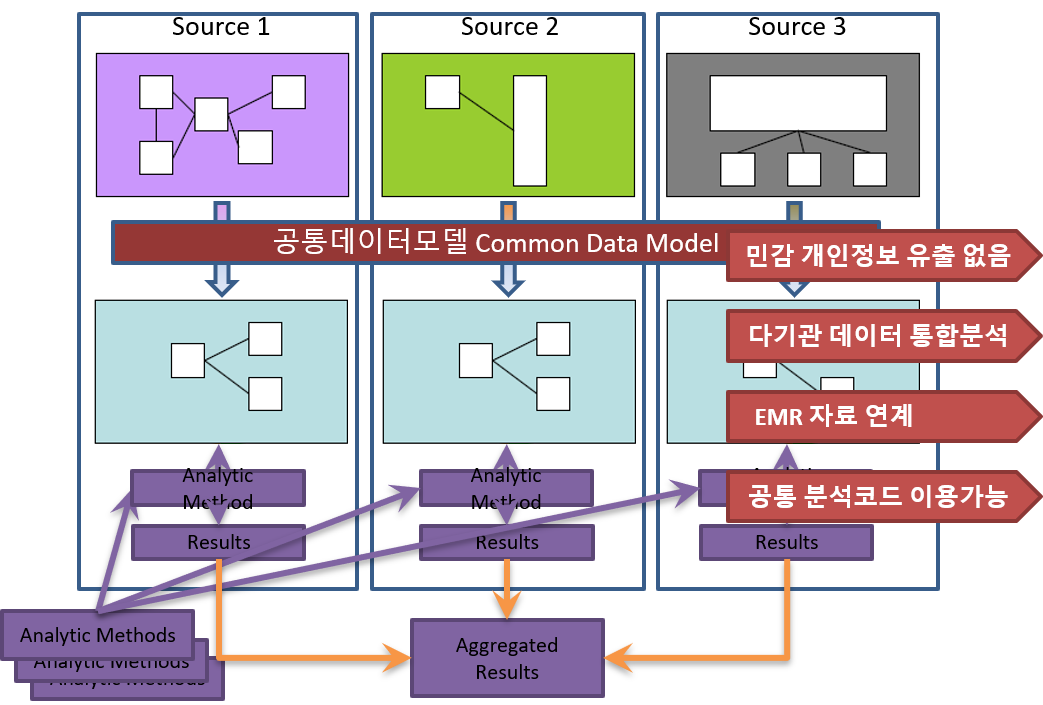
\includegraphics[width=0.75\linewidth]{images/OhdsiCommunity/CDM_DRN_1} \caption{Distributed Research Network}\label{fig:DRN}
\end{figure}

대표적인 공통데이터모델로는 비영리 국제컨소시엄인 오딧세이(Observational Health Data and Informatics, 이하 OHDSI)와 약물부작용 조사를 위한 미국 FDA의 센티넬 공통데이터모델(이하 Sentinel CDM), 미국 국내에서의 비교효과연구를 위한 피코르넷(The National Patient-Centered Clinical Outcomes Research Network, 이하 PCORnet) 등이 존재한다.

이중 대표적인 공통데이터모델인 OHDSI를 살펴보자. OHDSI는 2008년에 미국정부의 지원으로 결성된 Observational Medical Outcomes Partnership(OMOP)으로부터 파생된 국제적 협의체이다. 초기에는 관찰연구 방법론과 데이터를 활용하기 위한 분석 도구 및 시각화 도구, 그리고, 각 기관마다 다른 진단, 처방 용어를 통일한 표준용어를 만들었다.

OMOP은 2013년 정부의 지원이 예정대로 종료된 후, OMOP CDM과 표준 용어 정의 등 OHDSI로 이관되어 계속되고 있다. 특히 OMOP시절에는 약물부작용 조사 방법론에 초점을 맞추었지만, 이후 OHDSI로 이관한 이후에는 약물의 안전성, 비교효과연구, 경제성 분석, 의료의 질, 인공지능 기반의 환자 개별 위험도 예측 등 임상 빅데이터 분석으로 진화해 나가고 있다.

또 다른 CDM인 Sentinel Initiative는 미국 식품의약국(Food and Drug Administration, 이하 FDA)로부터 시작되었다. 의료 제품의 안전성 감시를 위한 국가적 전자시스템으로 Sentinel 시스템을 개발하였다. 이 시스템은 FDA 규제 제품을 사용하여 보고된 이상 반응을 추적하는 기존의 감시 기능을 보완하여 FDA가 이러한 제품의 안전성을 사전에 평가할 수 있도록 한다.

Sentinel은 데이터 파트너가 기존 환경에서 전자 데이터에 대한 물리적 및 운영상의 제어를 유지하는 분산 데이터 접근 방식을 사용한다. 분산된 접근 방식은 Sentinel CDM으로 저장된다. 참여하는 데이터 파트너는 자신들이 보유한 데이터를 통일된 Sentinel CDM으로 변환하므로 하나의 동일한 분석 프로그램으로 여러 기관 결과를 동시에 분석할 수 있다. 개인정보보호를 위하여 분석 쿼리가 배포되고 검색 결과가 보안 포털을 통해 반환된다. 모든 데이터 파트너들 사이에서 합쳐진 데이터 집합을 Sentinel Distributed Database(SDD)라고 한다.

또 다른 CDM인 PCORnet은 The Patient-Centered Outcomes Research Institute(PCORI)에서 2013년에 설립한 프로젝트로서 환자 전자건강기록(Electronic health records, EHR)을 이용하여 비교효과연구(Comparative effectiveness research, CER)를 수행하기 위한 목적으로 시작되었다. 50개 주에 걸쳐 11개의 임상 데이터 연구 네트워크(Clinical data research networks, CDRNs)와 18개의 환자 참여 연구 네트워크(Patient-powered research networks, PPRNs)를 설립했다. PCORnet이 구축하고 있는 연구 플랫폼의 핵심은 환자 중심의 접근 방식(patient-centered approach)이며 데이터는 중추 역할을 한다.

\hypertarget{OHDSINetwork}{%
\section{오딧세이 네트워크 (OHDSI network)}\label{OHDSINetwork}}

오딧세이 네트워크 (The Observational Health Data Sciences and Informatics, OHDSI network)는 의약품의 적절한 사용에 대한 관찰 연구의 증진을 위해 시작된 OMOP (Observational Medical Outcomes Partnership) 프로젝트를 전신으로 하여 만들어진 국제 컨소시엄이다. 공통데이터모델 (CDM) 및 분산연구망 (Distributed Research Network)을 채택한 연구 네트워크 중 아시아, 미국 및 유럽 등 국제적 참여 및 활동이 이루어 지고 있는 컨소시엄은 OHDSI가 유일하다. OHDSI 네트워크에서는 OMOP-CDM을 채택하여, 이를 발전시켜 나가고 있으며 국제적 연구자들의 적극적인 참여, 협력 및 토론과 함께 데이터 시각화, 분석 등의 소프트웨어를 개발 및 제공하고 있다.

\hypertarget{OHDSIHistory}{%
\section{OHDSI의 역사}\label{OHDSIHistory}}

2008년 미국 식약처 (FDA) 주도로 공공기관과 여러 제약회사, 의료기관을 포함하는 민간기관, 학계가 합동하여 후향적 보건 데이터베이스의 적절한 활용을 통해 의약품의 효과 및 안정성을 확인하기 위한 파트너십으로 OMOP (Observational Medical Outcomes Partnership) 프로젝트가 시작되었다 \href{https://fnih.org/what-we-do/major-completed-programs/omop}{ref}. 2009년 \href{http://forums.ohdsi.org/uploads/default/original/1X/7b3fb0f7acda70533b966d2834fef4ded62a97be.docx}{OMOP-CDM version 1}이 탄생하였다 \href{http://forums.ohdsi.org/t/is-omop-cdm-10-years-old-in-2017/3370/4}{ref}. OMOP은 common data model (CDM) 인프라 기반으로 청구 데이터 (claim data) 및 전자 의무 기록 (eletronic heatlh record) 를 통합하고 대규모 통계 분석의 가능성 및 유용성을 확인하였고, 2013년 Reagan-Udall 재단으로 이전되었다.
FDA의 재정 지원이 중단된 후 OMOP은 해체되었지만, Columbia 대학을 조직 본부 (coordinating center), George Hripsack 교수를 의장으로 하여 프로젝트에 참여했던 사람들은 다시 오픈 사이언스를 지향하는 비영리 연구 네트워크 오딧세이 (OHDSI) 를 구성하였다. 원래는 긴 여정을 뜻하는 ODYSSEY로 이름을 짓고 싶었지만, 너무 많은 단체에서 사용하고 있는 이름이어서 사전의 영문 발음기호를 따라 OHDSI라고 지었다는 후문이 전해진다.
2014년 뉴욕 Columbia 대학에서 Face-to-Face 모임 (F2F meeting)을 가진 후 2015년 워싱턴 (Washington DC)에서 첫번째 연례 심포지엄을 가졌다. 이후 매년 워싱턴 또는 베데스타 (Bethesda) 에서 가을에 연례 심포지엄을 열고 있다. OHDSI의 가치에 따라 연례 심포지엄은 무료로 진행이 되고 있다.

\hypertarget{OHDSIKoreaHistory}{%
\subsection{한국 오딧세이의 역사}\label{OHDSIKoreaHistory}}

아주대학교 박래웅 교수가 아주대 병원의 전자의무기록을 이용하여 2014년 OMOP-CDM 도입을 시작하였고, 2015년 첫 연례 심포지엄에서 활용 결과를 발표하면서 한국의 OHDSI 참여가 시작되었다. 이후 계속적으로 한국에서 OMOP-CDM, OHDSI 전파를 위해 노력하였고, 2016년부터는 최초로 국제 OHDSI committee에서 개별 국가를 위한 포럼 \href{http://forums.ohdsi.org/c/For-collaborators-wishing-to-communicate-in-Korean}{Korean chapter}을 개설하고, 한국의 OHDSI 참여를 독려하였다.
첫 한국 국제 오딧세이 심포지엄은 2017년 3월 아주대학교에서 튜토리얼, 리더십 미팅을 포함하여 3일간 개최되었다.

\begin{figure}
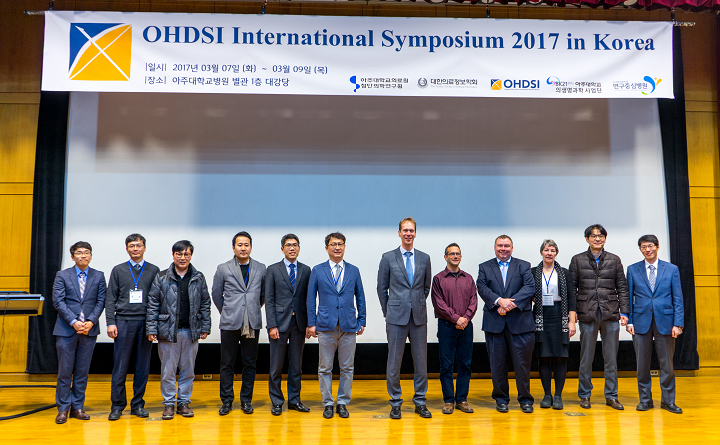
\includegraphics[width=0.8\linewidth]{images/OhdsiCommunity/DSC01956} \caption{OHDSI International Symposium 2017 in Korea}\label{fig:OHDSIInternationalSymposium2017inKorea1}
\end{figure}
\begin{figure}
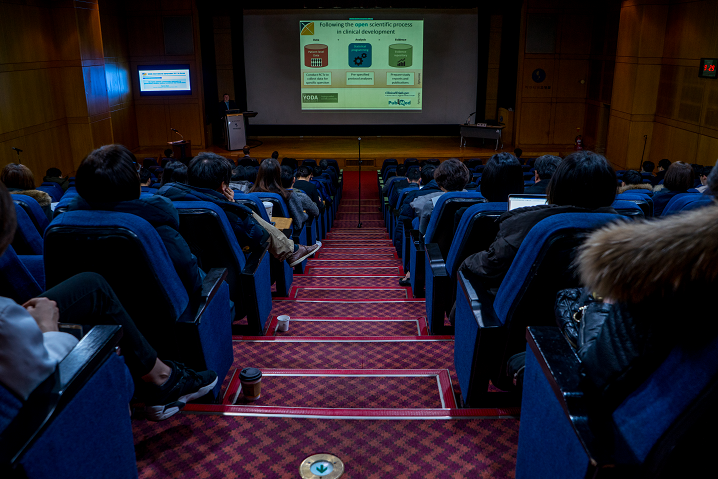
\includegraphics[width=0.8\linewidth]{images/OhdsiCommunity/DSC01861} \caption{OHDSI International Symposium 2017 in Korea}\label{fig:OHDSIInternationalSymposium2017inKorea1}
\end{figure}

\begin{figure}
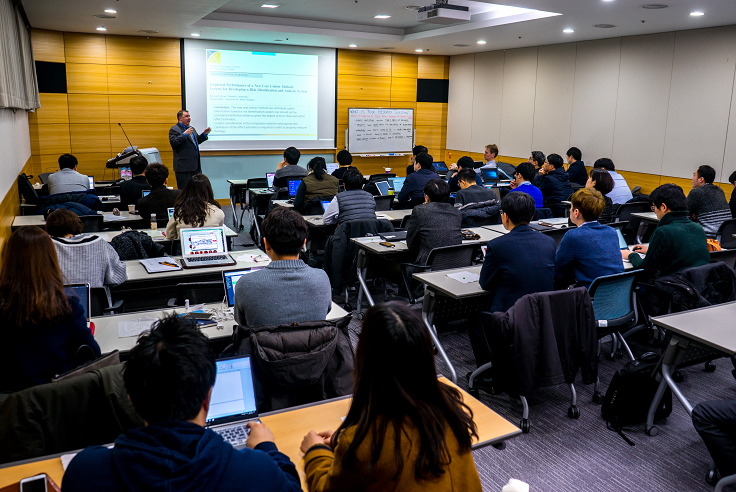
\includegraphics[width=0.8\linewidth]{images/OhdsiCommunity/DSC02166} \caption{Tutorial in the OHDSI International Symposium 2017}\label{fig:OHDSIInternationalSymposium2017inKorea2}
\end{figure}

한국 OHDSI 네트워크에 참여를 희망하는 병원 관계자들과 함께 2017년 3월 7일 첫번째 리더십 미팅을 가진 후 현재까지 2달마다 전국의 의과대학/병원을 순회하며 한국 OHDSI 리더십 미팅을 개최하며 OHDSI 전파 및 상호 협력을 꾀하고 있다.

\hypertarget{MissionVissionValues}{%
\section{미션, 비젼, 가치}\label{MissionVissionValues}}

\href{https://www.ohdsi.org/who-we-are/mission-vision-values/}{OHDSI 공식 홈페이지의 mission, vision, value page}에서 확인할 수 있다.

\hypertarget{ohdsi--1}{%
\subsection{OHDSI 미션}\label{ohdsi--1}}

참여 공동체의 상호협력 하에 의료 발전을 촉진하는 증거를 생성하는 능력을 부여한다.

\begin{quote}
To improve health by empowering a community to collaboratively generate the evidence that promotes better health decisions and better care.
\end{quote}

\hypertarget{ohdsi--2}{%
\subsection{OHDSI 비전}\label{ohdsi--2}}

의료 빅데이터의 분석을 통해 세계에 건강과 질병에 대한 포괄적인 이해를 제공한다.

\begin{quote}
A world in which observational research produces a comprehensive understanding of health and disease.
\end{quote}

\hypertarget{ohdsi--}{%
\subsection{OHDSI 핵심 가치}\label{ohdsi--}}

\begin{itemize}
\tightlist
\item
  \textbf{혁신성 Innovation}: 우리는 적극적으로 의료 빅데이터 분석 및 연구에 대한 혁신적인 방법론과 접근법을 찾고 격려한다.
\end{itemize}

\begin{quote}
Observational research is a field which will benefit greatly from disruptive thinking. We actively seek and encourage fresh methodological approaches in our work.
\end{quote}

\begin{itemize}
\tightlist
\item
  \textbf{재현성 Reproducibility}: 우리는 보건 증진을 위하여 정확하고, 재현 가능하며, 잘 보정된 증거를 찾도록 노력한다.
\end{itemize}

\begin{quote}
Accurate, reproducible, and well-calibrated evidence is necessary for health improvement.
\end{quote}

\begin{itemize}
\tightlist
\item
  \textbf{공동체 정신 Community}: 우리는 모든 참여자들을 환영하며 동등하게 우리의 활동에 참여할 수 있도록 돕는다.
\end{itemize}

\begin{quote}
Everyone is welcome to actively participate in OHDSI, whether you are a patient, a health professional, a researcher, or someone who simply believes in our cause.
\end{quote}

\begin{itemize}
\tightlist
\item
  \textbf{개방성 Openness}: 우리는 의사 결정 과정의 투명성을 지향하며, 우리의 진보 및 우리가 생성한 방법론, 소프트웨어, 증거를 가능한 공개적으로 접근 가능하게 한다.
\end{itemize}

\begin{quote}
We strive to make all our community's proceeds open and publicly accessible, including the methods, tools and the evidence that we generate.
\end{quote}

\begin{itemize}
\tightlist
\item
  \textbf{협력 정신 Collaboration}: 우리는 참여자들의 실제적 요구를 우선적으로 다루고, 그것을 위해 공동으로 노력한다.
\end{itemize}

\begin{quote}
We work collectively to prioritize and address the real world needs of our community's participants.
\end{quote}

\begin{itemize}
\tightlist
\item
  \textbf{선행의 정신 Beneficence}: 우리는 고통 받는 환자를 비롯하여 참여자 및 참여기관의 권리를 보호하기 위해 노력한다.
\end{itemize}

\begin{quote}
We seek to protect the rights of individuals and organizations within our community at all times.
\end{quote}

OHDSI의 핵심 가치를 요약해 보면, `개방적인 커뮤니티에서 함께 혁신적이고, 재현 가능한 연구를 통해 선행의 정신을 구현하자' 정도로 요약해볼 수 있겠다.

\hypertarget{ReproducibleResearch}{%
\section{재현 가능한 연구 (Open Science and Reproducible Research)}\label{ReproducibleResearch}}

OHDSI하면 전세계적에 통용 가능한 CDM 기반의 DRN 시스템이 가장 큰 특징으로 꼽히겠지만, 그 못지 않게 중요한 특징은 개방성과 재현성을 추구한다는 데에 있다.

\hypertarget{reproducibility-crisis}{%
\subsection{연구 재현성의 위기 (Reproducibility Crisis)}\label{reproducibility-crisis}}

2016년 Nature지에서 1576명을 대상으로 설문조사를 진행하였을 때, 70\% 이상의 연구자들이 다른 사람의 실험을 재현하는 데 실패하였으며, 약 50\%에서 자신의 실험을 재현하는 데 실패했다고 밝혔다. 52\%의 연구자들은 현재 과학계에 중대한 재현성의 위기가 존재한다고 시인했다. \href{https://www.nature.com/news/1-500-scientists-lift-the-lid-on-reproducibility-1.19970}{ref}

\begin{figure}
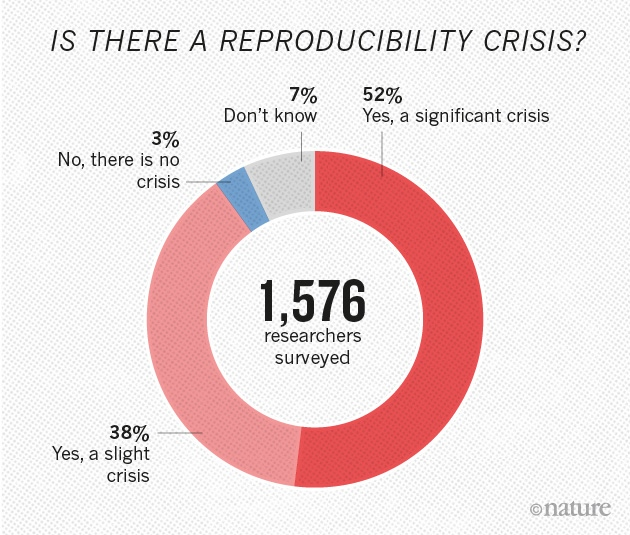
\includegraphics[width=0.8\linewidth]{images/OhdsiCommunity/reproducibility-graphic-online1} \caption{연구 재현성의 위기는 실존하는가?}\label{fig:isThereAReproducibilityCrisis}
\end{figure}

의료 데이터를 이용한 재현 가능한 연구 (Reproducible research)를 아주 간단히 정의하자면 '원 자료 (raw data)로부터 같은 결과를 도출하는 데이터 분석'이라고 할 수 있다.

유전자 데이터 및 의료 의무기록 등의 급증과 더불어 부상하고 있는 의료계의 빅데이터 분석 흐름에, 많은 연구들이 거짓 증거들을 만들고 있는 것이 아닌가하는 우려가 뒤따르고 있다. 실제로 PLOS Medicine에 실린 논문에 따르면 연구 대상자 수가 충분치 않은 역학 연구의 경우 1/10 경우만이 믿을 수 있고, 논문을 위한 논문 (Discovery-oriented exploratory research with massive testing)의 경우 1000개 중 1개 만이 믿을만 하다고 한다 {[}ref, \emph{Ioannidis, 2005 PLOS Medicine}{]}.

\begin{figure}
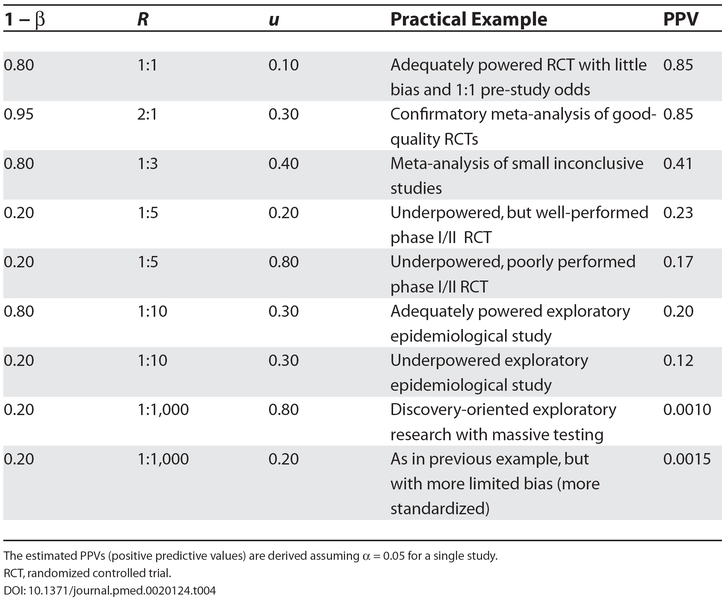
\includegraphics[width=0.8\linewidth]{images/OhdsiCommunity/journal.pmed.0020124.t004} \caption{PPV of Research Findings for various combinations of power, ratio of Tru to Not-True Relationship, and Bias}\label{fig:whyMostPublishedResarchFindingsAreFalse}
\end{figure}

어째서 이러한 일이 벌어지고 있는 것일까? 연구 재현성을 가로막는 것으로는 다음의 4가지가 주요 요인으로 꼽힌다{[}ref, \emph{Bishop, 2019, Nature}{]}.

\begin{itemize}
\tightlist
\item
  출판 편향 Publication Bias
\item
  충분치 않은 연구 대상자 수 또는 낮은 위험도 비 Low Statistical Power
\item
  \emph{P} 값 해킹 \emph{P}-value Hacking
\item
  결과를 알고 난 후 가설 재 수립 HARKing (Hypothesizing After Results are Known)
\end{itemize}

\hypertarget{publication-bias}{%
\subsubsection{출판 편향 Publication Bias}\label{publication-bias}}

\emph{많은 관심을 받는 선택 편향의 또 다른 버전은 출퍈 편향이다. 출판 편향이란 어떤 현상을 보여주는 데 실패했다는 논문보다 성공했다는 논문을 과학 저널이 더 선호하는 경향이 있다는 것이다. 이 경향은 '서류함 효과 (file drawer effect)로도 불린다. 이 명칭은, 일부 연구 결과는 논문으로 완성되어 과학 저널에 실리지 못하고 끝내 서류함 속에 머문다는 뜻을 담고 있다.}
{[}ref, 데이비드 핸드, 신은 주사위 놀이를 하지 않는다. 165쪽{]}

출판 편향은 p-value hacking 및 HARKing을 일으키는 근본 원인이 된다. 현재 한국 연구 사회는 논문의 impact factor (IF) 를 이용하여 연구자의 자질을 평가하고, 줄을 세우고 있기 때문에 세상에 기여를 하는 연구보다는 높은 IF의 논문이 연구자들의 주요 목적이 되고 있다.

\hypertarget{low-statistical-power}{%
\subsubsection{충분치 않은 연구 대상자 수 또는 낮은 위험도 비 Low Statistical Power}\label{low-statistical-power}}

연구의 대상 샘플 크기가 적거나 (small sample size) 효과의 크기가 적은 경우 (small effect), 위양성의 결과가 나올 가능성이 높다. 충분한 수를 갖지 못한 (underpowered) 연구를 지속하는 원동력은 원하는 결과가 나오길 바라는 맹목적인 바람뿐이고, 이는 낭비나 다름 없다는 {[}ref, R. G. Newcombe Br. Med. J. (Clin. Res. Ed.) 295, 656--659; 1987{]} 주장도 있다. Low Statistical Power를 지닌 연구를 진행하면서, 출판 편향을 극복하기 위해 통계적으로 유의미한 결과를 내기 위해 결국 \emph{p}-value hacking과 HARKing이 사용될 수밖에 없다. 하지만 이는 결국 맹목적으로 IF 성과를 요구하는 연구 사회의 태도와 이러한 결과를 인정해주는 연구 풍토에서 기인한다고 볼 수 있다.

\hypertarget{p----------p-value-hacking-and-harking-hypothesizing-after-results-are-known}{%
\subsubsection{\texorpdfstring{\emph{P} 값 해킹과 결과를 알고 난 후 가설 재 수립 \emph{P}-value Hacking and HARKing (Hypothesizing After Results are Known)}{P 값 해킹과 결과를 알고 난 후 가설 재 수립 P-value Hacking and HARKing (Hypothesizing After Results are Known)}}\label{p----------p-value-hacking-and-harking-hypothesizing-after-results-are-known}}

\emph{P}-value hacking 및 HARKing 은 많은 연구자에게 만연하게 나타나고 있는 현상으로, `Discovery-oriented exploratory research with massive testing'이라고도 부를 수 있다. 높은 IF의 저널에 출판하기 위하여 통계학적으로 유의한 결과가 중요해짐에 따라, 연구자들은 어떤 방식으로든 통계학적으로 유의미한 \emph{P}-value (\emph{P} \textless{} 0.05) 를 만들어내는 경향이 있고, 데이터 수집 및 분석을 다양히 시도해봄으로써 어떠한 결과도 만들어 낼 수 있다. 'False-Positive Psychology' 제목의 논문에서 Simmons 등은 4가지의 자유도 (변수, 샘플 크기, 공변량 사용, 보고하고 싶은 결과)를 자유롭게 선택할 수 있다면 `비틀즈의 노래를 듣고 나면 나이가 어려진다' 라는 황당한 결론을 만들어내는 것도 가능하다는 것을 입증했다 {[}ref, Simmons et al., 2011 Psychological Science{]}. \href{https://projects.fivethirtyeight.com/p-hacking/}{Hack Your Ways To Scientific Glory} 사이트는 \emph{P}-hacking 시뮬레이션을 제공하는데, 실제 여러변 testing을 거치며 0.05 미만의 \emph{P} 값을 찾아내는 우리의 현실과 매우 유사하다.

\hypertarget{section}{%
\subsection{재현가능한 연구를 위하여}\label{section}}

Simmons 등은 앞선 연구에서 연구의 위양성을 줄이기 위하여 하기와 같이, 6가지의 공개 중심 방안 (disclosure based solution)을 소개했다. 간단히 정리 하자면 데이터를 투명하게 수집하고, 충분한 샘플 크기를 가지고, 사용하는 변수와 방법, 그리고 결과를 모두 공개하라는 것이다.

\begin{verbatim}
1. Authors must decide the rules for the terminating data collection before data collectino begins and report this rules in the article
2. Authors must collect at least 20 observations per cell or else provide a compelling cost-of-data collection justification
3. Authors must list all variables collected in a study
4. Authors must report all experimental conditions, including failed manipulations
5. If observation are elimiated, authors must also report what the statistical results are if those observations are included
6. If an analysis includes a covariate, authors must report the statistical results of the analysis without the covariate. 
\end{verbatim}

강제는 아니지만 연구 재현성을 위한 OHDSI 연구의 기본 철학은 `파이프라인과 같은 연구' 이다. 데이터베이스로부터 결과 도출까지의 전 과정을 자동화하는 것을 목표로 하고 있다. OHDSI에서 연구를 수행한다는 것은 결국 이러한 파이프라인을 만드는 작업이 된다. 이러한 정신에 입각하여 연구에 사용된 코드를 \href{https://github.com/OHDSI/OhdsiStudies}{OHDSI Studies GitHub} 또는 \href{https://github.com/OHDSI/StudyProtocols}{OHDSI Study Protocol Github}을 통해 모두 공개하며 \href{http://data.ohdsi.org/}{연구 결과} 역시 공개하고 있다.

\begin{figure}
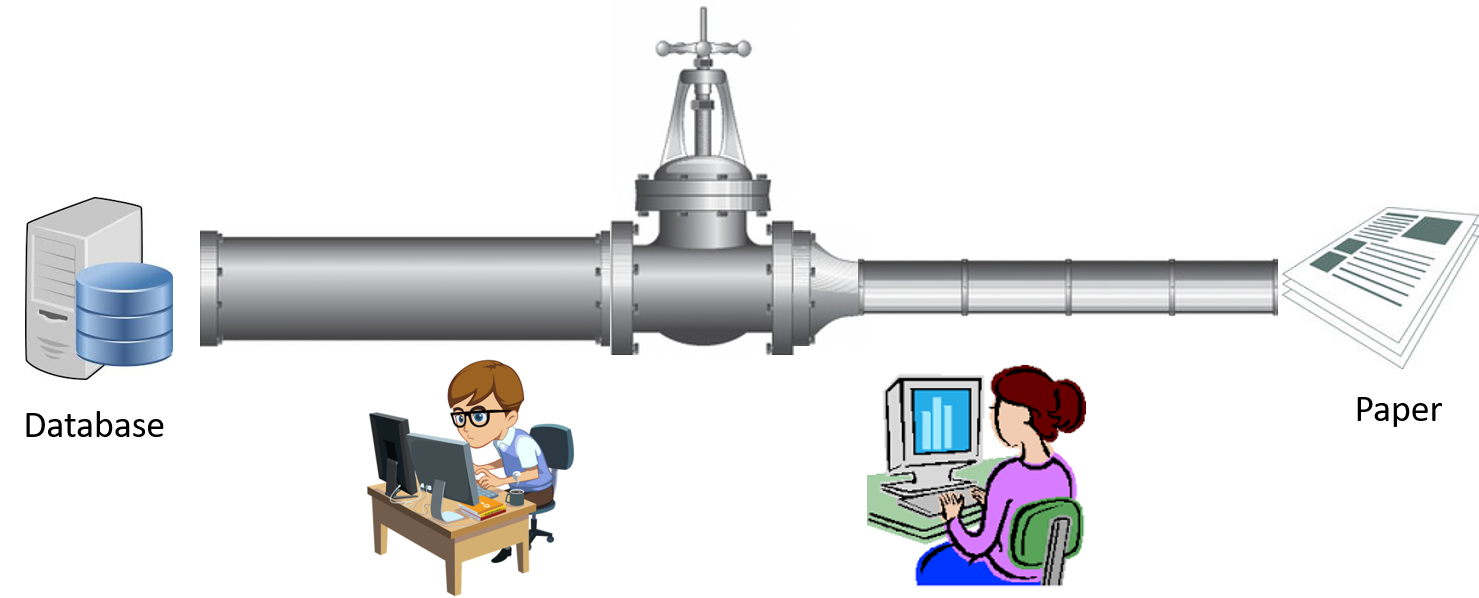
\includegraphics[width=0.8\linewidth]{images/OhdsiCommunity/study_pipeline} \caption{An OHDSI study shoul be look like a pipeline}\label{fig:ohdsiStudyShouldBeLookLikeAPipeline}
\end{figure}

\hypertarget{omopCdm}{%
\chapter{The OMOP-CDM}\label{omopCdm}}

\begin{itemize}
\tightlist
\item
  최신 OMOP-CDM 상세설명서 : \href{https://github.com/ohdsi/commondatamodel/wiki}{CDM wiki page}에서 가장 최신의 OMOP-CDM 공식 상세 설명을 보실 수 있습니다.
\item
  OMOP-CDM Github : \href{https://github.com/ohdsi/commondatamodel}{OMOP-CDM github}
\item
  OMOP-CDM 이슈 페이지 : OMOP-CDM 발전에 대한 건의사항은 \href{https://github.com/ohdsi/commondatamodel/issues}{OMOP-CDM 이슈페이지}에 올리면 된다.
\item
  OHDSI tutorial : \href{https://www.ohdsi.org/past-events/}{OHDSI past event}에서 \href{https://www.ohdsi.org/past-events/2018-tutorials-omop-common-data-model-and-standardized-vocabularies/}{영문 OMOP-CDM tutorial}을 보실 수 있다.
\end{itemize}

\hypertarget{section-1}{%
\section{설계 원칙}\label{section-1}}

OMOP-CDM은 신뢰성 있는 보건 과학적 증거를 발견하는데 필요한 관찰 의료 데이터의 속성들을 가급적 모두 포함하기 위하여 설계되었다. OMOP-CDM의 설계 원칙은 하기와 같다.

\begin{itemize}
\tightlist
\item
  \textbf{Suitability for purpose:} The CDM aims to provide data organized in a way optimal for analysis, rather than for the purpose of addressing the operational needs of health care providers or payers.
\item
  \textbf{Data protection:} All data that might jeopardize the identity and protection of patients, such as names, precise birthdays etc. are limited. Exceptions are possible where the research expressly requires more detailed information, such as precise birth dates for the study of infants.
\item
  \textbf{Design of domains:} The domains are modeled in a person-centric relational data model, where for each record the identity of the person and a date is captured as a minimum.
\item
  \textbf{Rationale for domains:} Domains are identified and separately defined in an entity-relationship model if they have an analysis use case and the domain has specific attributes that are not otherwise applicable. All other data can be preserved as an observation in an entity-attribute-value structure.
\item
  \textbf{Standardized Vocabularies:} To standardize the content of those records, the CDM relies on the Standardized Vocabularies containing all necessary and appropriate corresponding standard healthcare concepts.
\item
  \textbf{Reuse of existing vocabularies:} If possible, these concepts are leveraged from national or industry standardization or vocabulary definition organizations or initiatives, such as the National Library of Medicine, the Department of Veterans' Affairs, the Center of Disease Control and Prevention, etc.
\item
  \textbf{Maintaining source codes:} Even though all codes are mapped to the Standardized Vocabularies, the model also stores the original source code to ensure no information is lost.
\item
  \textbf{Technology neutrality:} The CDM does not require a specific technology. It can be realized in any relational database, such as Oracle, SQL Server etc., or as SAS analytical datasets.
\item
  \textbf{Scalability:} The CDM is optimized for data processing and computational analysis to accommodate data sources that vary in size, including databases with up to hundreds of millions of persons and billions of clinical observations.
\item
  \textbf{Backwards compatibility:} All changes from previous CDMs are clearly delineated in the github repository \href{https://github.com/OHDSI/CommonDataModel}{(https://github.com/OHDSI/CommonDataModel)}. Older versions of the CDM can be easily created from the CDMv5, and no information is lost that was present previously.
\end{itemize}

\hypertarget{data-model-conventions}{%
\section{Data Model Conventions}\label{data-model-conventions}}

There are a number of implicit and explicit conventions that have been adopted in the CDM. Developers of methods that run against the CDM need to understand these conventions.

\hypertarget{model-conv}{%
\subsection{General conventions of the model}\label{model-conv}}

The OMOP CDM is considered a ``person-centric'' model, meaning that the people (or patients) drive the event and observation tables. At a minimum, the tables have a foreign key into the PERSON table and a date. This allows for a longitudinal view on all healthcare-relevant events by person. The exceptions from this rule are the standardized health system data tables, which are linked directly to events of the various domains.

\hypertarget{general-conventions-of-schemas}{%
\subsection{General conventions of schemas}\label{general-conventions-of-schemas}}

New to CDM v6.0 is the concept of schemas. This allows for more separation between read-only and writeable tables. The clinical data, event, and vocabulary tables are in the `CDM' schema and are considered read-only to the end user. This means that the tables can be queried but no information can be accidentally removed or written over except by the database administrator. Tables that need to be manipulated by web-based tools or end users have moved to the `Results' schema. Currently the only two tables in the `Results' schema are COHORT and COHORT\_DEFINITON, \textbf{add a sentence explaining that these tables describe groups of interest that the user might define, put in links to the later sections} though likely more will be added over the course of v6.0 point releases. These tables can be written to, meaning that a cohort created in ATLAS or by a user can be stored in the COHORT table and accessed at a later date. This does mean that cohorts in the COHORT table can be manipulated by anyone so it is always recommended that the SQL code used to create the cohort be saved along with the project or analysis in the event it needs to be regenerated.

\hypertarget{general-conventions-of-data-tables}{%
\subsection{General conventions of data tables}\label{general-conventions-of-data-tables}}

The CDM is platform-independent. Data types are defined generically using ANSI SQL data types (VARCHAR, INTEGER, FLOAT, DATE, DATETIME, CLOB). Precision is provided only for VARCHAR. It reflects the minimal required string length and can be expanded within a CDM instantiation. The CDM does not prescribe the date and datetime format. Standard queries against CDM may vary for local instantiations and date/datetime configurations.

In most cases, the first field in each table ends in '\_ID', containing a record identifier that can be used as a foreign key in another table. For example, the CONDITION\_OCCURRENCE table contains the field VISIT\_OCCURRENCE\_ID which is a foreign key to the VISIT\_OCCURRENCE table where VISIT\_OCCURRENCE\_ID is the primary key.

\hypertarget{general-conventions-of-fields}{%
\subsection{General conventions of fields}\label{general-conventions-of-fields}}

Variable names across all tables follow one convention:

\begin{longtable}[]{@{}ll@{}}
\toprule
\begin{minipage}[b]{0.24\columnwidth}\raggedright
Notation\strut
\end{minipage} & \begin{minipage}[b]{0.71\columnwidth}\raggedright
Description\strut
\end{minipage}\tabularnewline
\midrule
\endhead
\begin{minipage}[t]{0.24\columnwidth}\raggedright
\_SOURCE\_VALUE\strut
\end{minipage} & \begin{minipage}[t]{0.71\columnwidth}\raggedright
Verbatim information from the source data, typically used in ETL to map to CONCEPT\_ID, and not to be used by any standard analytics. For example, CONDITION\_SOURCE\_VALUE = `787.02' was the ICD-9 code captured as a diagnosis from the administrative claim.\strut
\end{minipage}\tabularnewline
\begin{minipage}[t]{0.24\columnwidth}\raggedright
\_ID\strut
\end{minipage} & \begin{minipage}[t]{0.71\columnwidth}\raggedright
Unique identifiers for key entities, which can serve as foreign keys to establish relationships across entities. For example, PERSON\_ID uniquely identifies each individual. VISIT\_OCCURRENCE\_ID uniquely identifies a PERSON encounter at a point of care.\strut
\end{minipage}\tabularnewline
\begin{minipage}[t]{0.24\columnwidth}\raggedright
\_CONCEPT\_ID\strut
\end{minipage} & \begin{minipage}[t]{0.71\columnwidth}\raggedright
Foreign key into the Standardized Vocabularies (i.e.~the standard\_concept attribute for the corresponding term is true), which serves as the primary basis for all standardized analytics. For example, CONDITION\_CONCEPT\_ID = 31967 \href{http://athena.ohdsi.org/search-terms/terms/31967}{(http://athena.ohdsi.org/search-terms/terms/31967)} contains the reference value for the SNOMED concept of `Nausea'\strut
\end{minipage}\tabularnewline
\begin{minipage}[t]{0.24\columnwidth}\raggedright
\_SOURCE\_CONCEPT\_ID\strut
\end{minipage} & \begin{minipage}[t]{0.71\columnwidth}\raggedright
Foreign key into the Standardized Vocabularies representing the concept and terminology used in the source data, when applicable. For example, CONDITION\_SOURCE\_CONCEPT\_ID = 45431665 \href{http://athena.ohdsi.org/search-terms/terms/45431665}{(http://athena.ohdsi.org/search-terms/terms/45431665)} denotes the concept of `Nausea' in the Read terminology; the analogous CONDITION\_CONCEPT\_ID might be 31967, since SNOMED-CT is the Standardized Vocabulary for most clinical diagnoses and findings.\strut
\end{minipage}\tabularnewline
\begin{minipage}[t]{0.24\columnwidth}\raggedright
\_TYPE\_CONCEPT\_ID\strut
\end{minipage} & \begin{minipage}[t]{0.71\columnwidth}\raggedright
Delineates the origin of the source information, standardized within the Standardized Vocabularies. For example, DRUG\_TYPE\_CONCEPT\_ID can allow analysts to discriminate between `Pharmacy dispensing' and `Prescription written'\strut
\end{minipage}\tabularnewline
\bottomrule
\end{longtable}

\hypertarget{representation-of-content-through-concepts}{%
\subsection{Representation of content through Concepts}\label{representation-of-content-through-concepts}}

In CDM data tables the content of each record is represented using Concepts. Concepts are stored in event tables with their CONCEPT\_IDs as foreign keys to the CONCEPT table, which contains Concepts necessary to describe the healthcare experience of a patient. If a Standard Concept does not exist or cannot be identified, the the CONCEPT\_ID 0 is used, representing a non-existing concept or un-mappable source value.

Records in the CONCEPT table contain detailed information about each concept (name, domain, class etc.). Concepts, Concept Relationships, Concept Ancestors and other information relating to Concepts is contained in the tables of the Standardized Vocabularies.

\hypertarget{difference-between-concept-ids-and-source-values}{%
\subsection{Difference between Concept IDs and Source Values}\label{difference-between-concept-ids-and-source-values}}

Many tables contain equivalent information in multiple places: As a Source Value, a Source Concept and as a Standard Concept.

\begin{itemize}
\tightlist
\item
  Source Values contain the codes from public code systems such as ICD-9-CM, NDC, CPT-4, READ etc. or locally controlled vocabularies (such as F for female and M for male) copied from the source data. Source Values are stored in the \_SOURCE\_VALUE fields in the data tables.
\item
  Concepts are CDM-specific entities that represent the meaning of a clinical fact. Most concepts are based on code systems used in healthcare (called Source Concepts), while others were created de-novo (CONCEPT\_CODE = `OMOP generated'). Concepts have unique IDs across all domains.
\item
  Source Concepts are the concepts that represent the code used in the source. Source Concepts are only used for common healthcare code systems, not for OMOP-generated Concepts. Source Concepts are stored in the \_SOURCE\_CONCEPT\_ID field in the data tables.
\item
  Standard Concepts are those concepts that are used to define the unique meaning of a clinical entity. For each entity there is one Standard Concept. Standard Concepts are typically drawn from existing public vocabulary sources. Concepts that have the equivalent meaning to a Standard Concept are mapped to the Standard Concept. Standard Concepts are referred to in the \_CONCEPT\_ID field of the data tables.
\end{itemize}

Source Values are only provided for convenience and quality assurance (QA) purposes. Source Values and Source Concepts are optional, while \textbf{Standard Concepts are mandatory}. Source Values may contain information that is only meaningful in the context of a specific data source. This mandatory use of Standard Concepts is what allows all OHDSI collaborators to speak the same language. For example, let's look at the condition `Pulmonary Tuberculosis' (TB). Figure \ref{fig:pulmTubICD9} shows that the ICD9CM code for TB is 011.

\begin{figure}
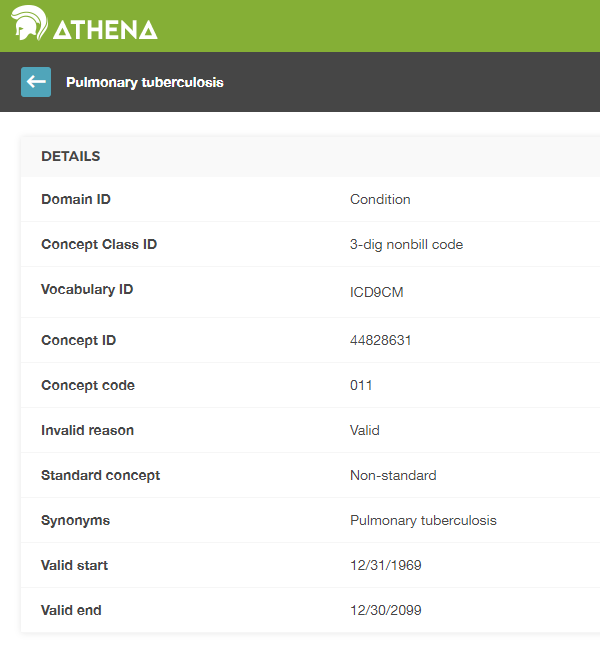
\includegraphics[width=0.75\linewidth]{images/CommonDataModel/pulmTubICD9} \caption{ICD9CM code for Pulmonary Tuberculosis}\label{fig:pulmTubICD9}
\end{figure}

Without the use of a standard way to represent TB the code 011 could be interpreted as `Hospital Inpatient (Including Medicare Part A)' in the UB04 vocabulary, or as `Nervous System Neoplasms without Complications, Comorbidities' in the DRG vocabulary. This is where Concept IDs, both Source and Standard, are valuable. The Concept ID that represents the 011 ICD9CM code is 44828631 \href{http://athena.ohdsi.org/search-terms/terms/44828631}{(http://athena.ohdsi.org/search-terms/terms/44828631)}. This differentiates the ICD9CM from the UBO4 and from the DRG. The Standard Concept that ICD9CM code maps to is 253954 \href{http://athena.ohdsi.org/search-terms/terms/253954}{(http://athena.ohdsi.org/search-terms/terms/253954)} as shown in figure \ref{fig:pulmTubMap} by the relationship `Non-standard to Standard map (OMOP)'. This same mapping relationship exists between Read, ICD10, CIEL, and MeSH codes, among others, so that any research that references the standard SNOMED concept is sure to include all supported source codes.

\begin{figure}
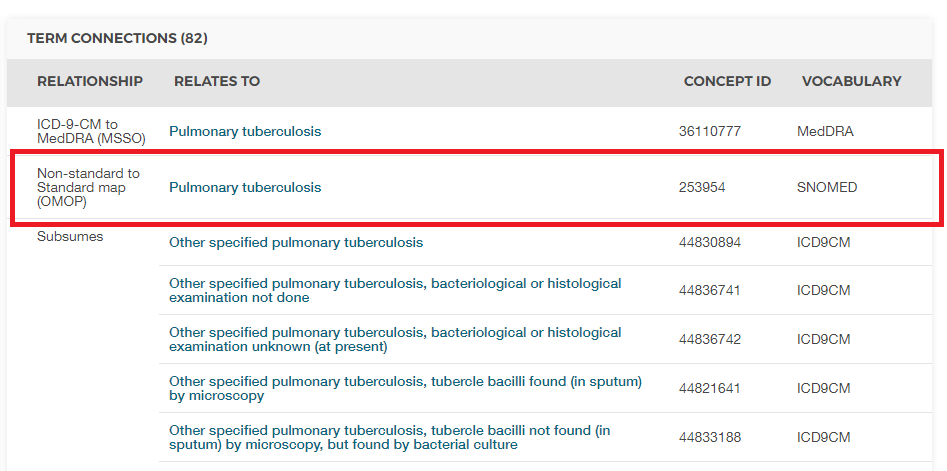
\includegraphics[width=1\linewidth]{images/CommonDataModel/pulmTubMap} \caption{SNOMED code for Pulmonary Tuberculosis}\label{fig:pulmTubMap}
\end{figure}

An example of how this relationship is depicted in the tables is shown in figure (\textbf{link to figure in CONDITION\_OCCURRENCE})

\hypertarget{omop-cdm-standardized-tables}{%
\section{OMOP CDM Standardized Tables}\label{omop-cdm-standardized-tables}}

The OMOP CDM contains 16 Clinical data tables, 10 Vocabulary tables, 2 Metadata tables, 4 Health System data tables, 2 Health Economics data tables, 3 standardized derived elements, and 2 results schema tables. To illustrate how these tables are utilized in practice the data of one person will be used as a common thread throughout the rest of the chapter. While part of the CDM the Vocabulary tables are not covered here, rather, they are detailed in depth in Chapter \ref{StandardizedVocabularies}.

\hypertarget{omop-cdm----table-specification}{%
\subsection{OMOP-CDM 의 상세 설명 (table specification)}\label{omop-cdm----table-specification}}

OMOP-CDM은 \href{https://github.com/ohdsi/commondatamodel}{OHDSI Common Data Model 깃헙}에서 관리되고 있다. 2019년 5월 25일 현재 기준으로 모델 버전은 6.0이다. 모델이 자주 업데이트 되므로 최신 버전에 대해서는 깃헙 의 \href{https://github.com/OHDSI/CommonDataModel/wiki}{wiki page} 에서 확인하는 것이 좋다. 이전 버전의 OMOP-CDM specification이 필요할 경우 깃헙의 Tags에서 원하는 버전으로 이동한 후 pdf 파일을 열어 보면 된다.

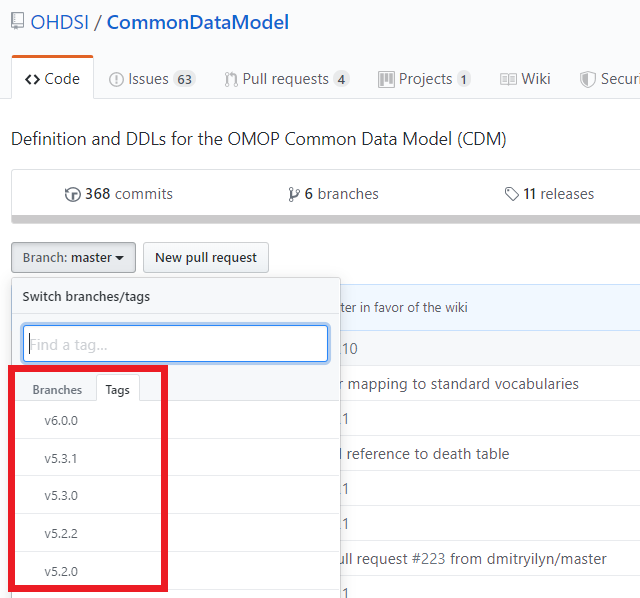
\includegraphics[width=0.8\linewidth]{images/CommonDataModel/github_tags}
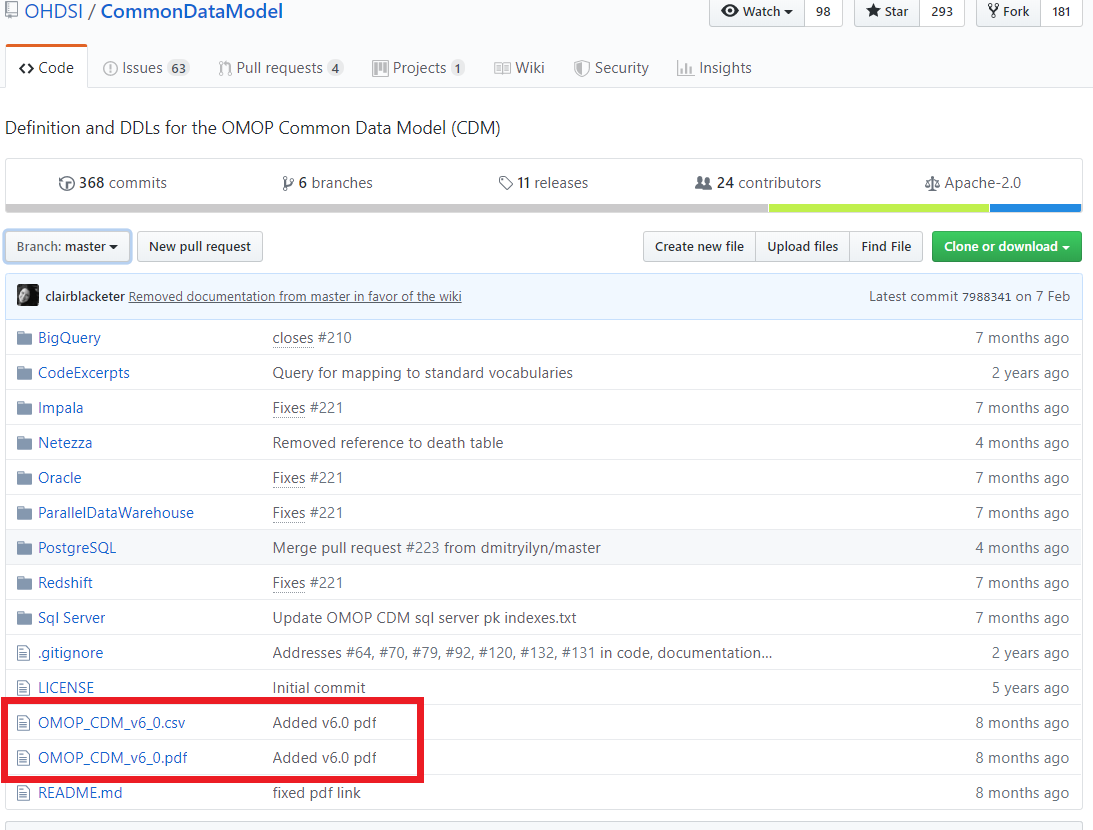
\includegraphics[width=0.8\linewidth]{images/CommonDataModel/github_pdf}

\hypertarget{omop-cdm----}{%
\subsection{OMOP-CDM 건의 사항 및 업그레이드}\label{omop-cdm----}}

Open community로 운영되는 OHDSI에서 OMOP-CDM 의 진화 역시 사용자에 의해서 결정된다. 만약, OMOP-CDM의 데이터 아키텍처에 대해 건의사항이 있을 경우 CDM \href{https://github.com/ohdsi/commondatamodel/issues}{깃헙}에 의견을 자유롭게 적을 수 있다. OMOP-CDM 운영자들은 이를 확인하고 다른 사람들과 의논, 필요시 투표하여 차후의 버전에 필요사항을 반영할 것이다.

OMOP-CDM 구조는 진화 중이며, 2019년 5월 30일 기준 최신 버전은 v6.0 이다.

\begin{figure}
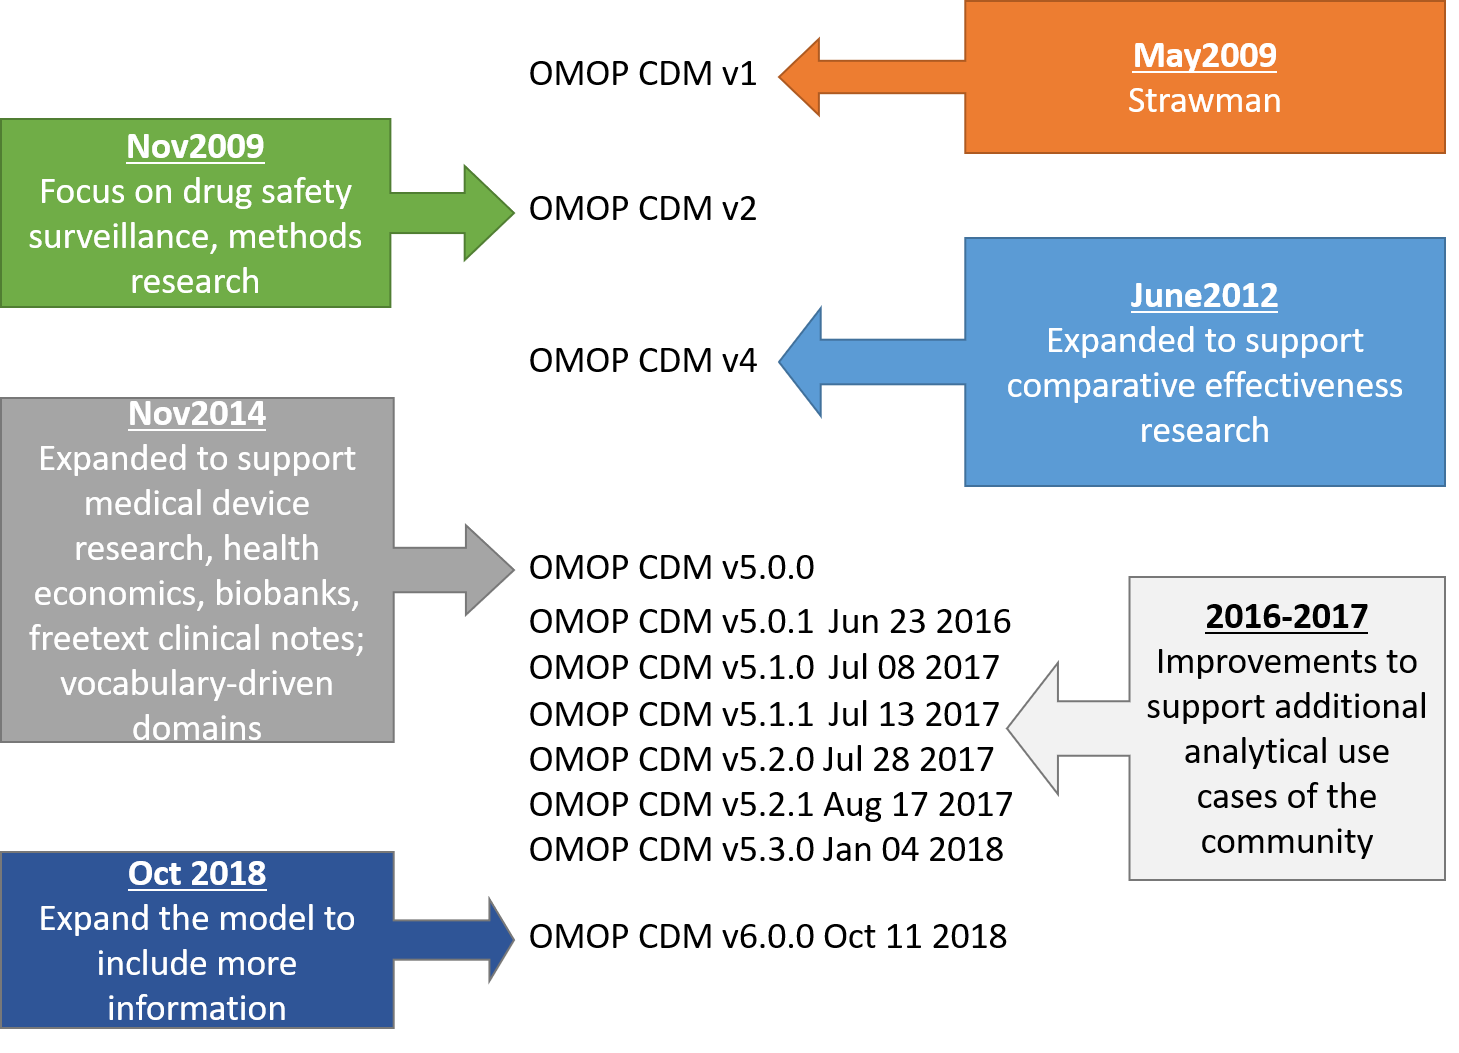
\includegraphics[width=0.8\linewidth]{images/CommonDataModel/history_of_CDM} \caption{Evolution of OMOP-CDM}\label{fig:cdmHistory}
\end{figure}

\hypertarget{running-example-endometriosis}{%
\subsection{Running Example: Endometriosis}\label{running-example-endometriosis}}

Endometriosis is a painful condition whereby cells normally found in the lining of a woman's uterus occur elsewhere in the body. Severe cases can lead to infertility, bowel, and bladder problems. The following sections will detail one patient's experience with this disease and how her clinical experience might be represented in the Common Data Model.

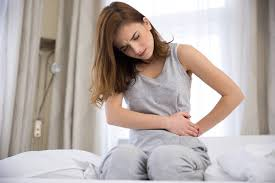
\includegraphics[width=0.5\linewidth]{images/CommonDataModel/Lauren}

\begin{figure}
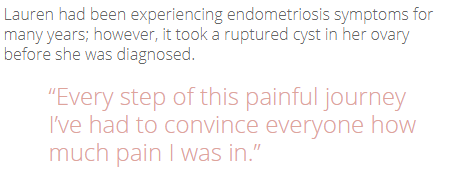
\includegraphics[width=0.75\linewidth]{images/CommonDataModel/laurentext} \caption{Read more about Lauren and endometriosis at https://www.endometriosis-uk.org/laurens-story}\label{fig:Laurentext}
\end{figure}

\hypertarget{person}{%
\subsection{PERSON table}\label{person}}

As the Common Data Model is a person-centric model (see section \ref{model-conv}) let's start with how she would be represented in the PERSON table. For the full PERSON table specification please see the CDM wiki \url{https://github.com/OHDSI/CommonDataModel/wiki/PERSON}.

\textbf{What do we know about Lauren?}

\begin{itemize}
\tightlist
\item
  She is a 36-year-old woman
\item
  Her birthday is 12-March-1982
\item
  She is white
\item
  She is english
\end{itemize}

With that in mind, her PERSON table might look something like this:

\begin{longtable}[]{@{}lll@{}}
\toprule
\begin{minipage}[b]{0.33\columnwidth}\raggedright
Column Name\strut
\end{minipage} & \begin{minipage}[b]{0.15\columnwidth}\raggedright
Value\strut
\end{minipage} & \begin{minipage}[b]{0.43\columnwidth}\raggedright
Explanation\strut
\end{minipage}\tabularnewline
\midrule
\endhead
\begin{minipage}[t]{0.33\columnwidth}\raggedright
person\_id\strut
\end{minipage} & \begin{minipage}[t]{0.15\columnwidth}\raggedright
1\strut
\end{minipage} & \begin{minipage}[t]{0.43\columnwidth}\raggedright
Person\_id should be an integer, either directly from the source or generated as part of the build process.\strut
\end{minipage}\tabularnewline
\begin{minipage}[t]{0.33\columnwidth}\raggedright
gender\_concept\_id\strut
\end{minipage} & \begin{minipage}[t]{0.15\columnwidth}\raggedright
8532\strut
\end{minipage} & \begin{minipage}[t]{0.43\columnwidth}\raggedright
The concept\_id referring to female gender is 8532 \href{http://athena.ohdsi.org/search-terms/terms/8532}{(http://athena.ohdsi.org/search-terms/terms/8532)}.\strut
\end{minipage}\tabularnewline
\begin{minipage}[t]{0.33\columnwidth}\raggedright
year\_of\_birth\strut
\end{minipage} & \begin{minipage}[t]{0.15\columnwidth}\raggedright
1982\strut
\end{minipage} & \begin{minipage}[t]{0.43\columnwidth}\raggedright
\strut
\end{minipage}\tabularnewline
\begin{minipage}[t]{0.33\columnwidth}\raggedright
month\_of\_birth\strut
\end{minipage} & \begin{minipage}[t]{0.15\columnwidth}\raggedright
3\strut
\end{minipage} & \begin{minipage}[t]{0.43\columnwidth}\raggedright
\strut
\end{minipage}\tabularnewline
\begin{minipage}[t]{0.33\columnwidth}\raggedright
day\_of\_birth\strut
\end{minipage} & \begin{minipage}[t]{0.15\columnwidth}\raggedright
12\strut
\end{minipage} & \begin{minipage}[t]{0.43\columnwidth}\raggedright
\strut
\end{minipage}\tabularnewline
\begin{minipage}[t]{0.33\columnwidth}\raggedright
birth\_datetime\strut
\end{minipage} & \begin{minipage}[t]{0.15\columnwidth}\raggedright
1982-03-12 00:00:00\strut
\end{minipage} & \begin{minipage}[t]{0.43\columnwidth}\raggedright
When the time is not known midnight is used.\strut
\end{minipage}\tabularnewline
\begin{minipage}[t]{0.33\columnwidth}\raggedright
death\_datetime\strut
\end{minipage} & \begin{minipage}[t]{0.15\columnwidth}\raggedright
\strut
\end{minipage} & \begin{minipage}[t]{0.43\columnwidth}\raggedright
\strut
\end{minipage}\tabularnewline
\begin{minipage}[t]{0.33\columnwidth}\raggedright
race\_concept\_id\strut
\end{minipage} & \begin{minipage}[t]{0.15\columnwidth}\raggedright
8527\strut
\end{minipage} & \begin{minipage}[t]{0.43\columnwidth}\raggedright
The concept\_id referring to white race is 8527 \href{http://athena.ohdsi.org/search-terms/terms/8527}{(http://athena.ohdsi.org/search-terms/terms/8527)}.\strut
\end{minipage}\tabularnewline
\begin{minipage}[t]{0.33\columnwidth}\raggedright
ethnicity\_concept\_id\strut
\end{minipage} & \begin{minipage}[t]{0.15\columnwidth}\raggedright
38003564\strut
\end{minipage} & \begin{minipage}[t]{0.43\columnwidth}\raggedright
Typically hispanic status is stored for ethnicity. The concept\_id 38003564 \href{http://athena.ohdsi.org/search-terms/terms/38003564}{(http://athena.ohdsi.org/search-terms/terms/38003564)} refers to `Not hispanic'.\strut
\end{minipage}\tabularnewline
\begin{minipage}[t]{0.33\columnwidth}\raggedright
location\_id\strut
\end{minipage} & \begin{minipage}[t]{0.15\columnwidth}\raggedright
\strut
\end{minipage} & \begin{minipage}[t]{0.43\columnwidth}\raggedright
Her address is not known.\strut
\end{minipage}\tabularnewline
\begin{minipage}[t]{0.33\columnwidth}\raggedright
provider\_id\strut
\end{minipage} & \begin{minipage}[t]{0.15\columnwidth}\raggedright
\strut
\end{minipage} & \begin{minipage}[t]{0.43\columnwidth}\raggedright
Her primary care provider is not known.\strut
\end{minipage}\tabularnewline
\begin{minipage}[t]{0.33\columnwidth}\raggedright
care\_site\_id\strut
\end{minipage} & \begin{minipage}[t]{0.15\columnwidth}\raggedright
\strut
\end{minipage} & \begin{minipage}[t]{0.43\columnwidth}\raggedright
Her primary care site is not known.\strut
\end{minipage}\tabularnewline
\begin{minipage}[t]{0.33\columnwidth}\raggedright
person\_source\_value\strut
\end{minipage} & \begin{minipage}[t]{0.15\columnwidth}\raggedright
1\strut
\end{minipage} & \begin{minipage}[t]{0.43\columnwidth}\raggedright
Typically this would be her identifier in the source data, though often is it the same as the person\_id.\strut
\end{minipage}\tabularnewline
\begin{minipage}[t]{0.33\columnwidth}\raggedright
gender\_source\_value\strut
\end{minipage} & \begin{minipage}[t]{0.15\columnwidth}\raggedright
F\strut
\end{minipage} & \begin{minipage}[t]{0.43\columnwidth}\raggedright
The gender value as it appears in the source is stored here.\strut
\end{minipage}\tabularnewline
\begin{minipage}[t]{0.33\columnwidth}\raggedright
gender\_source\_concept\_id\strut
\end{minipage} & \begin{minipage}[t]{0.15\columnwidth}\raggedright
0\strut
\end{minipage} & \begin{minipage}[t]{0.43\columnwidth}\raggedright
If the gender value in the source was coded using a vocabulary recognized by OHDSI, that concept\_id would go here. For example, if her gender was `Sex-F' in the source and it was stated to be in the PCORNet vocabulary concept\_id 44814665 \href{http://athena.ohdsi.org/search-terms/terms/44814665}{(http://athena.ohdsi.org/search-terms/terms/44814665)} would go in this field.\strut
\end{minipage}\tabularnewline
\begin{minipage}[t]{0.33\columnwidth}\raggedright
race\_source\_value\strut
\end{minipage} & \begin{minipage}[t]{0.15\columnwidth}\raggedright
white\strut
\end{minipage} & \begin{minipage}[t]{0.43\columnwidth}\raggedright
The race value as it appears in the source is stored here.\strut
\end{minipage}\tabularnewline
\begin{minipage}[t]{0.33\columnwidth}\raggedright
race\_source\_concept\_id\strut
\end{minipage} & \begin{minipage}[t]{0.15\columnwidth}\raggedright
0\strut
\end{minipage} & \begin{minipage}[t]{0.43\columnwidth}\raggedright
Same principle as gender\_source\_concept\_id.\strut
\end{minipage}\tabularnewline
\begin{minipage}[t]{0.33\columnwidth}\raggedright
ethnicity\_source\_value\strut
\end{minipage} & \begin{minipage}[t]{0.15\columnwidth}\raggedright
english\strut
\end{minipage} & \begin{minipage}[t]{0.43\columnwidth}\raggedright
The ethnicity value as it appears in the source is stored here.\strut
\end{minipage}\tabularnewline
\begin{minipage}[t]{0.33\columnwidth}\raggedright
ethnicity\_source\_concept\_id\strut
\end{minipage} & \begin{minipage}[t]{0.15\columnwidth}\raggedright
0\strut
\end{minipage} & \begin{minipage}[t]{0.43\columnwidth}\raggedright
Same principle as gender\_source\_concept\_id.\strut
\end{minipage}\tabularnewline
\bottomrule
\end{longtable}

\hypertarget{observationPeriod}{%
\subsection{OBSERVATION\_PERIOD table}\label{observationPeriod}}

The OBSERVATION\_PERIOD table is designed to define the amount of time for which a patient's clinical events are recorded in the source system. For US healthcare insurance claims this is typically the enrollment period of the patient. When working with data from electronic health records (EHR) often the first record in the system is considered the observation\_period\_start\_date and the latest record is considered the observation\_period\_end\_date with the understanding that only the clinical events that happened within that particular system were recorded. For the full OBSERVATION\_PERIOD table specification please see the CDM wiki \href{https://github.com/OHDSI/CommonDataModel/wiki/OBSERVATION_PERIOD}{(https://github.com/OHDSI/CommonDataModel/wiki/OBSERVATION\_PERIOD)}.

\textbf{How can we determine Lauren's observation period?}

Lauren's information is most similar to EHR data in that we only have records of her encounters from which to determine her observation period.

\begin{longtable}[]{@{}llll@{}}
\toprule
Encounter\_ID & Start\_Date & Stop\_Date & EncounterClass\tabularnewline
\midrule
\endhead
70 & 2010-01-06 & 2010-01-06 & outpatient\tabularnewline
80 & 2011-01-06 & 2011-01-06 & outpatient\tabularnewline
90 & 2012-01-06 & 2012-01-06 & outpatient\tabularnewline
100 & 2013-01-07 & 2013-01-07 & outpatient\tabularnewline
101 & 2013-01-14 & 2013-01-14 & ambulatory\tabularnewline
102 & 2013-01-17 & 2013-01-24 & inpatient\tabularnewline
\bottomrule
\end{longtable}

Based on the encounter records her OBSERVATION\_PERIOD table might look something like this:

\begin{longtable}[]{@{}lll@{}}
\toprule
\begin{minipage}[b]{0.33\columnwidth}\raggedright
Column Name\strut
\end{minipage} & \begin{minipage}[b]{0.15\columnwidth}\raggedright
Value\strut
\end{minipage} & \begin{minipage}[b]{0.43\columnwidth}\raggedright
Explanation\strut
\end{minipage}\tabularnewline
\midrule
\endhead
\begin{minipage}[t]{0.33\columnwidth}\raggedright
observation\_period\_id\strut
\end{minipage} & \begin{minipage}[t]{0.15\columnwidth}\raggedright
1\strut
\end{minipage} & \begin{minipage}[t]{0.43\columnwidth}\raggedright
This is typically an autogenerated field that creates a unique id number for each record in the table.\strut
\end{minipage}\tabularnewline
\begin{minipage}[t]{0.33\columnwidth}\raggedright
person\_id\strut
\end{minipage} & \begin{minipage}[t]{0.15\columnwidth}\raggedright
1\strut
\end{minipage} & \begin{minipage}[t]{0.43\columnwidth}\raggedright
This comes from the PERSON table and links PERSON and OBSERVATION\_PERIOD.\strut
\end{minipage}\tabularnewline
\begin{minipage}[t]{0.33\columnwidth}\raggedright
observation\_period\_start\_date\strut
\end{minipage} & \begin{minipage}[t]{0.15\columnwidth}\raggedright
2010-01-06\strut
\end{minipage} & \begin{minipage}[t]{0.43\columnwidth}\raggedright
This is the start date of her earliest encounter on record.\strut
\end{minipage}\tabularnewline
\begin{minipage}[t]{0.33\columnwidth}\raggedright
observation\_period\_end\_date\strut
\end{minipage} & \begin{minipage}[t]{0.15\columnwidth}\raggedright
2013-01-24\strut
\end{minipage} & \begin{minipage}[t]{0.43\columnwidth}\raggedright
This is the end date of her latest encounter on record.\strut
\end{minipage}\tabularnewline
\begin{minipage}[t]{0.33\columnwidth}\raggedright
period\_type\_concept\_id\strut
\end{minipage} & \begin{minipage}[t]{0.15\columnwidth}\raggedright
44814725\strut
\end{minipage} & \begin{minipage}[t]{0.43\columnwidth}\raggedright
The best option in the Vocabulary with the concept class `Obs Period Type' is 44814724 \href{http://athena.ohdsi.org/search-terms/terms/44814724}{(http://athena.ohdsi.org/search-terms/terms/44814724)}, which stands for `Period covering healthcare encounters'.\strut
\end{minipage}\tabularnewline
\bottomrule
\end{longtable}

\hypertarget{visitOccurrence}{%
\subsection{VISIT\_OCCURRENCE}\label{visitOccurrence}}

The VISIT\_OCCURRENCE table houses information about a patient's encounters with the health care system. Within the OHDSI vernacular these are referred to as visits and are considered to be discreet events. There are 12 categories of visits though the most common are inpatient, outpatient, emergency and long term care. For the full VISIT\_OCCURRENCE table specification please see the CDM wiki \href{https://github.com/OHDSI/CommonDataModel/wiki/VISIT_OCCURRENCE}{(https://github.com/OHDSI/CommonDataModel/wiki/VISIT\_OCCURRENCE)}.

\textbf{How do we represent Lauren's encounters as visits?}

Revisting the encounters we used to determine her observation period:

\begin{longtable}[]{@{}llll@{}}
\toprule
Encounter\_ID & Start\_Date & Stop\_Date & EncounterClass\tabularnewline
\midrule
\endhead
70 & 2010-01-06 & 2010-01-06 & outpatient\tabularnewline
80 & 2011-01-06 & 2011-01-06 & outpatient\tabularnewline
90 & 2012-01-06 & 2012-01-06 & outpatient\tabularnewline
100 & 2013-01-07 & 2013-01-07 & outpatient\tabularnewline
101 & 2013-01-14 & 2013-01-14 & ambulatory\tabularnewline
\textbf{102} & \textbf{2013-01-17} & \textbf{2013-01-24} & \textbf{inpatient}\tabularnewline
\bottomrule
\end{longtable}

As an example let's represent the inpatient encounter as a record in the VISIT\_OCCURRENCE table.

\begin{longtable}[]{@{}lll@{}}
\toprule
\begin{minipage}[b]{0.25\columnwidth}\raggedright
Column Name\strut
\end{minipage} & \begin{minipage}[b]{0.17\columnwidth}\raggedright
Value\strut
\end{minipage} & \begin{minipage}[b]{0.50\columnwidth}\raggedright
Explanation\strut
\end{minipage}\tabularnewline
\midrule
\endhead
\begin{minipage}[t]{0.25\columnwidth}\raggedright
visit\_occurrence\_id\strut
\end{minipage} & \begin{minipage}[t]{0.17\columnwidth}\raggedright
514\strut
\end{minipage} & \begin{minipage}[t]{0.50\columnwidth}\raggedright
This is typically an autogenerated field that creates a unique id number for each visit on the person's record in the converted CDM database.\strut
\end{minipage}\tabularnewline
\begin{minipage}[t]{0.25\columnwidth}\raggedright
person\_id\strut
\end{minipage} & \begin{minipage}[t]{0.17\columnwidth}\raggedright
1\strut
\end{minipage} & \begin{minipage}[t]{0.50\columnwidth}\raggedright
This comes from the PERSON table and links PERSON and VISIT\_OCCURRENCE.\strut
\end{minipage}\tabularnewline
\begin{minipage}[t]{0.25\columnwidth}\raggedright
visit\_concept\_id\strut
\end{minipage} & \begin{minipage}[t]{0.17\columnwidth}\raggedright
9201\strut
\end{minipage} & \begin{minipage}[t]{0.50\columnwidth}\raggedright
The concept\_id referring to an inpatient visit is 9201 \href{http://athena.ohdsi.org/search-terms/terms/9201}{(http://athena.ohdsi.org/search-terms/terms/9201)}.\strut
\end{minipage}\tabularnewline
\begin{minipage}[t]{0.25\columnwidth}\raggedright
visit\_start\_date\strut
\end{minipage} & \begin{minipage}[t]{0.17\columnwidth}\raggedright
2013-01-17\strut
\end{minipage} & \begin{minipage}[t]{0.50\columnwidth}\raggedright
The start date of the visit.\strut
\end{minipage}\tabularnewline
\begin{minipage}[t]{0.25\columnwidth}\raggedright
visit\_start\_datetime\strut
\end{minipage} & \begin{minipage}[t]{0.17\columnwidth}\raggedright
2013-01-17 00:00:00\strut
\end{minipage} & \begin{minipage}[t]{0.50\columnwidth}\raggedright
The date and time of the visit started. When time is unknown midnight is used.\strut
\end{minipage}\tabularnewline
\begin{minipage}[t]{0.25\columnwidth}\raggedright
visit\_end\_date\strut
\end{minipage} & \begin{minipage}[t]{0.17\columnwidth}\raggedright
2013-01-24\strut
\end{minipage} & \begin{minipage}[t]{0.50\columnwidth}\raggedright
The end date of the visit. If this is a one-day visit the end date should match the start date.\strut
\end{minipage}\tabularnewline
\begin{minipage}[t]{0.25\columnwidth}\raggedright
visit\_end\_datetime\strut
\end{minipage} & \begin{minipage}[t]{0.17\columnwidth}\raggedright
2013-01-24 00:00:00\strut
\end{minipage} & \begin{minipage}[t]{0.50\columnwidth}\raggedright
The date and time of the visit end. If time is unknown midnight is used.\strut
\end{minipage}\tabularnewline
\begin{minipage}[t]{0.25\columnwidth}\raggedright
visit\_type\_concept\_id\strut
\end{minipage} & \begin{minipage}[t]{0.17\columnwidth}\raggedright
32034\strut
\end{minipage} & \begin{minipage}[t]{0.50\columnwidth}\raggedright
This column is intended to provide information about the provenance of the visit record, i.e.~does it come from an insurance claim, hospital billing record, EHR record, etc. For this example the concept\_id 32035 \href{http://athena.ohdsi.org/search-terms/terms/32035}{(http://athena.ohdsi.org/search-terms/terms/32035)} is used as the encounters are similar to electronic health records\strut
\end{minipage}\tabularnewline
\begin{minipage}[t]{0.25\columnwidth}\raggedright
provider\_id*\strut
\end{minipage} & \begin{minipage}[t]{0.17\columnwidth}\raggedright
NULL\strut
\end{minipage} & \begin{minipage}[t]{0.50\columnwidth}\raggedright
If the encounter record has a provider associated, the id for that provider goes in this field. This should be the provider\_id from the PROVIDER table that represents the provider on the encounter.\strut
\end{minipage}\tabularnewline
\begin{minipage}[t]{0.25\columnwidth}\raggedright
care\_site\_id\strut
\end{minipage} & \begin{minipage}[t]{0.17\columnwidth}\raggedright
NULL\strut
\end{minipage} & \begin{minipage}[t]{0.50\columnwidth}\raggedright
If the encounter record has a care site associated, the id for that care site goes in this field. This should be the care\_site\_id from the CARE\_SITE table that codes for the care site on the encounter.\strut
\end{minipage}\tabularnewline
\begin{minipage}[t]{0.25\columnwidth}\raggedright
visit\_source\_value\strut
\end{minipage} & \begin{minipage}[t]{0.17\columnwidth}\raggedright
inpatient\strut
\end{minipage} & \begin{minipage}[t]{0.50\columnwidth}\raggedright
The visit value as it appears in the source goes here. In this context `visit' means outpatient, inpatient, emergency, etc.\strut
\end{minipage}\tabularnewline
\begin{minipage}[t]{0.25\columnwidth}\raggedright
visit\_source\_concept\_id\strut
\end{minipage} & \begin{minipage}[t]{0.17\columnwidth}\raggedright
0\strut
\end{minipage} & \begin{minipage}[t]{0.50\columnwidth}\raggedright
If the visit value from the source is coded using a vocabulary that is recognized by OHDSI, the concept\_id that represents the visit source value would go here.\strut
\end{minipage}\tabularnewline
\begin{minipage}[t]{0.25\columnwidth}\raggedright
admitted\_from\_concept\_id\strut
\end{minipage} & \begin{minipage}[t]{0.17\columnwidth}\raggedright
0\strut
\end{minipage} & \begin{minipage}[t]{0.50\columnwidth}\raggedright
If known, this is the concept\_id that represents where the patient was admitted from. This concept should have the concept class `Place of Service' and the domain `Visit'. For example, if a patient was admitted to the hospital from home, the concept\_id would be 8536 \href{http://athena.ohdsi.org/search-terms/terms/8536}{(http://athena.ohdsi.org/search-terms/terms/8536)}.\strut
\end{minipage}\tabularnewline
\begin{minipage}[t]{0.25\columnwidth}\raggedright
admitted\_from\_source\_value\strut
\end{minipage} & \begin{minipage}[t]{0.17\columnwidth}\raggedright
NULL\strut
\end{minipage} & \begin{minipage}[t]{0.50\columnwidth}\raggedright
This is the value from the source that represents where the patient was admitted from. Using the above example, this would be `home'.\strut
\end{minipage}\tabularnewline
\begin{minipage}[t]{0.25\columnwidth}\raggedright
discharge\_to\_concept\_id\strut
\end{minipage} & \begin{minipage}[t]{0.17\columnwidth}\raggedright
0\strut
\end{minipage} & \begin{minipage}[t]{0.50\columnwidth}\raggedright
If known, this is the concept\_id that represents where the patient was discharged to. This concept should have the concept class `Place of Service' and the domain `Visit'. For example, if a patient was released to an assisted living facility, the concept\_id would be 8615 \href{http://athena.ohdsi.org/search-terms/terms/8615}{(http://athena.ohdsi.org/search-terms/terms/8615)}.\strut
\end{minipage}\tabularnewline
\begin{minipage}[t]{0.25\columnwidth}\raggedright
discharge\_to\_source\_value\strut
\end{minipage} & \begin{minipage}[t]{0.17\columnwidth}\raggedright
0\strut
\end{minipage} & \begin{minipage}[t]{0.50\columnwidth}\raggedright
This is the value from the source that represents where the patient was discharged to. Using the above example, this would be `assisted living facility'.\strut
\end{minipage}\tabularnewline
\begin{minipage}[t]{0.25\columnwidth}\raggedright
preceding\_visit\_occurrence\_id\strut
\end{minipage} & \begin{minipage}[t]{0.17\columnwidth}\raggedright
NULL\strut
\end{minipage} & \begin{minipage}[t]{0.50\columnwidth}\raggedright
The visit\_occurrence\_id for the visit immediately preceding the current one in time for the patient.\strut
\end{minipage}\tabularnewline
\bottomrule
\end{longtable}

*A patient may interact with multiple health care providers during one visit, as is often the case with inpatient stays. These interactions can be recorded in the VISIT\_DETAIL table. While not covered in depth in this chapter, you can read more about the VISIT\_DETAIL table on the CDM wiki \href{https://github.com/OHDSI/CommonDataModel/wiki/VISIT_DETAIL}{(https://github.com/OHDSI/CommonDataModel/wiki/VISIT\_DETAIL)}

\hypertarget{conditionOccurrence}{%
\subsection{CONDITION\_OCCURRENCE}\label{conditionOccurrence}}

Records in the CONDITION\_OCCURRENCE table are diagnoses, signs, or symptoms of a condition either observed by a Provider or reported by the patient.

\textbf{What are Lauren's conditions?}

Revisiting her account she says ``About 3 years ago I noticed my periods, which had also been
painful, were getting increasingly more painful. I started
becoming aware of a sharp jabbing pain right by my colon and
feeling tender and bloated around my tailbone and lower pelvis
area. My periods had become so painful that I was missing 1-2
days of work a month. Painkillers sometimes dulled the pain,
but usually they didn't do much.''

The SNOMED code for painful menstruation cramps, otherwise known as dysmenorrhea, is 266599000. Let's see how that would be represented in the CONDITION\_OCCURRENCE table:

\begin{longtable}[]{@{}lll@{}}
\toprule
\begin{minipage}[b]{0.27\columnwidth}\raggedright
Column\strut
\end{minipage} & \begin{minipage}[b]{0.14\columnwidth}\raggedright
Value\strut
\end{minipage} & \begin{minipage}[b]{0.50\columnwidth}\raggedright
Explanation\strut
\end{minipage}\tabularnewline
\midrule
\endhead
\begin{minipage}[t]{0.27\columnwidth}\raggedright
condition\_occurrence\_id\strut
\end{minipage} & \begin{minipage}[t]{0.14\columnwidth}\raggedright
964\strut
\end{minipage} & \begin{minipage}[t]{0.50\columnwidth}\raggedright
This is typically an autogenerated field that creates a unique id number for each condition on the person's record in the converted CDM database.\strut
\end{minipage}\tabularnewline
\begin{minipage}[t]{0.27\columnwidth}\raggedright
person\_id\strut
\end{minipage} & \begin{minipage}[t]{0.14\columnwidth}\raggedright
1\strut
\end{minipage} & \begin{minipage}[t]{0.50\columnwidth}\raggedright
This comes from the PERSON table and links PERSON and CONDITION\_OCCURRENCE.\strut
\end{minipage}\tabularnewline
\begin{minipage}[t]{0.27\columnwidth}\raggedright
condition\_concept\_id\strut
\end{minipage} & \begin{minipage}[t]{0.14\columnwidth}\raggedright
194696\strut
\end{minipage} & \begin{minipage}[t]{0.50\columnwidth}\raggedright
The concept\_id that represents the SNOMED code 266599000 is 194696 \href{http://athena.ohdsi.org/search-terms/terms/194696}{(http://athena.ohdsi.org/search-terms/terms/194696)}\strut
\end{minipage}\tabularnewline
\begin{minipage}[t]{0.27\columnwidth}\raggedright
condition\_start\_date\strut
\end{minipage} & \begin{minipage}[t]{0.14\columnwidth}\raggedright
2010-01-06\strut
\end{minipage} & \begin{minipage}[t]{0.50\columnwidth}\raggedright
The date when the instance of the Condition is recorded.\strut
\end{minipage}\tabularnewline
\begin{minipage}[t]{0.27\columnwidth}\raggedright
condition\_start\_datetime\strut
\end{minipage} & \begin{minipage}[t]{0.14\columnwidth}\raggedright
2010-01-06 00:00:00\strut
\end{minipage} & \begin{minipage}[t]{0.50\columnwidth}\raggedright
The date and time when the instance of the Condition is recorded. Midnight is used when the time is unknown\strut
\end{minipage}\tabularnewline
\begin{minipage}[t]{0.27\columnwidth}\raggedright
condition\_end\_date\strut
\end{minipage} & \begin{minipage}[t]{0.14\columnwidth}\raggedright
NULL\strut
\end{minipage} & \begin{minipage}[t]{0.50\columnwidth}\raggedright
If known, this is the date when the instance of the Condition is considered to have ended.\strut
\end{minipage}\tabularnewline
\begin{minipage}[t]{0.27\columnwidth}\raggedright
condition\_end\_datetime\strut
\end{minipage} & \begin{minipage}[t]{0.14\columnwidth}\raggedright
NULL\strut
\end{minipage} & \begin{minipage}[t]{0.50\columnwidth}\raggedright
If known, this is the date and time when the instance of the Condition is considered to have ended.\strut
\end{minipage}\tabularnewline
\begin{minipage}[t]{0.27\columnwidth}\raggedright
condition\_type\_concept\_id\strut
\end{minipage} & \begin{minipage}[t]{0.14\columnwidth}\raggedright
32020\strut
\end{minipage} & \begin{minipage}[t]{0.50\columnwidth}\raggedright
This column is intended to provide information about the provenance of the condition, i.e.~does it come from an insurance claim, hospital billing record, EHR record, etc. For this example the concept\_id 32020 \href{http://athena.ohdsi.org/search-terms/terms/32020}{(http://athena.ohdsi.org/search-terms/terms/32020)} is used as the encounters are similar to electronic health records. Concept\_ids in this field should be in the `Condition Type' vocabulary.\strut
\end{minipage}\tabularnewline
\begin{minipage}[t]{0.27\columnwidth}\raggedright
condition\_status\_concept\_id\strut
\end{minipage} & \begin{minipage}[t]{0.14\columnwidth}\raggedright
0\strut
\end{minipage} & \begin{minipage}[t]{0.50\columnwidth}\raggedright
If known, the condition\_status\_concept\_id represents when and/or how the condition was diagnosed. For example, a condition could be an admitting diagnosis, in which case the concept\_id 4203942 \href{http://athena.ohdsi.org/search-terms/terms/4203942}{(http://athena.ohdsi.org/search-terms/terms/4203942)} would be used.\strut
\end{minipage}\tabularnewline
\begin{minipage}[t]{0.27\columnwidth}\raggedright
stop\_reason\strut
\end{minipage} & \begin{minipage}[t]{0.14\columnwidth}\raggedright
NULL\strut
\end{minipage} & \begin{minipage}[t]{0.50\columnwidth}\raggedright
If known, the reason that the Condition was no longer present, as indicated in the source data.\strut
\end{minipage}\tabularnewline
\begin{minipage}[t]{0.27\columnwidth}\raggedright
provider\_id\strut
\end{minipage} & \begin{minipage}[t]{0.14\columnwidth}\raggedright
NULL\strut
\end{minipage} & \begin{minipage}[t]{0.50\columnwidth}\raggedright
If the condition record has a diagnosing provider listed, the id for that provider goes in this field. This should be the provider\_id from the PROVIDER table that represents the provider on the encounter.\strut
\end{minipage}\tabularnewline
\begin{minipage}[t]{0.27\columnwidth}\raggedright
visit\_occurrence\_id\strut
\end{minipage} & \begin{minipage}[t]{0.14\columnwidth}\raggedright
509\strut
\end{minipage} & \begin{minipage}[t]{0.50\columnwidth}\raggedright
If known, this is the visit (represented as visit\_occurrence\_id taken from the VISIT\_OCCURRENCE table) during which the condition was diagnosed.\strut
\end{minipage}\tabularnewline
\begin{minipage}[t]{0.27\columnwidth}\raggedright
visit\_detail\_id\strut
\end{minipage} & \begin{minipage}[t]{0.14\columnwidth}\raggedright
NULL\strut
\end{minipage} & \begin{minipage}[t]{0.50\columnwidth}\raggedright
If known, this is the visit detail encounter (represented as visit\_detail\_id from the VISIT\_DETAIL table) during which the condition was diagnosed.\strut
\end{minipage}\tabularnewline
\begin{minipage}[t]{0.27\columnwidth}\raggedright
condition\_source\_value\strut
\end{minipage} & \begin{minipage}[t]{0.14\columnwidth}\raggedright
266599000\strut
\end{minipage} & \begin{minipage}[t]{0.50\columnwidth}\raggedright
This is the value from the source that represents the condition. In Lauren's case of dysmenorrhea the SNOMED code for that condition is stored here and the standard concept\_id mapped from that code is stored in CONDITION\_CONCEPT\_ID.\strut
\end{minipage}\tabularnewline
\begin{minipage}[t]{0.27\columnwidth}\raggedright
condition\_source\_concept\_id\strut
\end{minipage} & \begin{minipage}[t]{0.14\columnwidth}\raggedright
194696\strut
\end{minipage} & \begin{minipage}[t]{0.50\columnwidth}\raggedright
If the condition value from the source is coded using a vocabulary that is recognized by OHDSI, the concept\_id that represents that value would go here. In the example of dysmennorhea the source value is a SNOMED code so the concept\_id that represents that code is 194696. In this case it is the same as the condition\_concept\_id since the SNOMED vocabulary is the standard condition vocabulary\strut
\end{minipage}\tabularnewline
\begin{minipage}[t]{0.27\columnwidth}\raggedright
condition\_status\_source\_value\strut
\end{minipage} & \begin{minipage}[t]{0.14\columnwidth}\raggedright
0\strut
\end{minipage} & \begin{minipage}[t]{0.50\columnwidth}\raggedright
If the condition status value from the source is coded using a vocabulary that is recognized by OHDSI, the concept\_id that represents that source value would go here.\strut
\end{minipage}\tabularnewline
\bottomrule
\end{longtable}

\hypertarget{drugExposure}{%
\subsection{DRUG\_EXPOSURE}\label{drugExposure}}

The DRUG\_EXPOSURE captures records about the utilization of a Drug when ingested or otherwise introduced into the body. Drugs include prescription and over-the-counter medicines, vaccines, and large-molecule biologic therapies. Radiological devices ingested or applied locally do not count as Drugs.

Drug Exposure is inferred from clinical events associated with orders, prescriptions written, pharmacy dispensings, procedural administrations, and other patient-reported information.

\textbf{What are Lauren's drug exposures?}

We know that Lauren was given 60 acetaminophen 325mg oral tablets for 30 days (NDC code 69842087651) at her visit on 2010-01-06 to help with her dysmenorrhea pain. Here's how that might look in the DRUG\_EXPOSURE table:

\begin{longtable}[]{@{}lll@{}}
\toprule
\begin{minipage}[b]{0.30\columnwidth}\raggedright
Column\strut
\end{minipage} & \begin{minipage}[b]{0.14\columnwidth}\raggedright
Value\strut
\end{minipage} & \begin{minipage}[b]{0.48\columnwidth}\raggedright
Explanation\strut
\end{minipage}\tabularnewline
\midrule
\endhead
\begin{minipage}[t]{0.30\columnwidth}\raggedright
drug\_exposure\_id\strut
\end{minipage} & \begin{minipage}[t]{0.14\columnwidth}\raggedright
1001\strut
\end{minipage} & \begin{minipage}[t]{0.48\columnwidth}\raggedright
This is typically an autogenerated field that creates a unique id number for each drug\_exposure on the person's record in the converted CDM database.\strut
\end{minipage}\tabularnewline
\begin{minipage}[t]{0.30\columnwidth}\raggedright
person\_id\strut
\end{minipage} & \begin{minipage}[t]{0.14\columnwidth}\raggedright
1\strut
\end{minipage} & \begin{minipage}[t]{0.48\columnwidth}\raggedright
This comes from the PERSON table and links PERSON and DRUG\_EXPOSURE.\strut
\end{minipage}\tabularnewline
\begin{minipage}[t]{0.30\columnwidth}\raggedright
drug\_concept\_id\strut
\end{minipage} & \begin{minipage}[t]{0.14\columnwidth}\raggedright
1127433\strut
\end{minipage} & \begin{minipage}[t]{0.48\columnwidth}\raggedright
The NDC code for acetaminophen maps to the RxNorm code 313782 which is represented by the concept\_id 1127433 \href{http://athena.ohdsi.org/search-terms/terms/1127433}{(http://athena.ohdsi.org/search-terms/terms/1127433)}.\strut
\end{minipage}\tabularnewline
\begin{minipage}[t]{0.30\columnwidth}\raggedright
drug\_exposure\_start\_date\strut
\end{minipage} & \begin{minipage}[t]{0.14\columnwidth}\raggedright
2010-01-06\strut
\end{minipage} & \begin{minipage}[t]{0.48\columnwidth}\raggedright
The start date of the drug exposure\strut
\end{minipage}\tabularnewline
\begin{minipage}[t]{0.30\columnwidth}\raggedright
drug\_exposure\_start\_datetime\strut
\end{minipage} & \begin{minipage}[t]{0.14\columnwidth}\raggedright
2010-01-06 00:00:00\strut
\end{minipage} & \begin{minipage}[t]{0.48\columnwidth}\raggedright
The start date and time of the drug exposure. Midnight is used when the time is not known.\strut
\end{minipage}\tabularnewline
\begin{minipage}[t]{0.30\columnwidth}\raggedright
drug\_exposure\_end\_date\strut
\end{minipage} & \begin{minipage}[t]{0.14\columnwidth}\raggedright
2010-02-05\strut
\end{minipage} & \begin{minipage}[t]{0.48\columnwidth}\raggedright
The end date of the drug exposure. Depending on different sources, it could be a known or an inferred date and denotes the last day at which the patient was still exposed to the drug. In this case the end is inferred since we know Lauren had a 30 days supply.\strut
\end{minipage}\tabularnewline
\begin{minipage}[t]{0.30\columnwidth}\raggedright
drug\_exposure\_end\_datetime\strut
\end{minipage} & \begin{minipage}[t]{0.14\columnwidth}\raggedright
2010-02-05 00:00:00\strut
\end{minipage} & \begin{minipage}[t]{0.48\columnwidth}\raggedright
The end date and time of the drug exposure. Similar rules apply as to drug\_exposure\_end\_date. Midnight is used when time is unknown\strut
\end{minipage}\tabularnewline
\begin{minipage}[t]{0.30\columnwidth}\raggedright
verbatim\_end\_date\strut
\end{minipage} & \begin{minipage}[t]{0.14\columnwidth}\raggedright
NULL\strut
\end{minipage} & \begin{minipage}[t]{0.48\columnwidth}\raggedright
If the source provides an end date rather than just days supply that date goes here.\strut
\end{minipage}\tabularnewline
\begin{minipage}[t]{0.30\columnwidth}\raggedright
drug\_type\_concept\_id\strut
\end{minipage} & \begin{minipage}[t]{0.14\columnwidth}\raggedright
38000177\strut
\end{minipage} & \begin{minipage}[t]{0.48\columnwidth}\raggedright
This column is intended to provide information about the provenance of the drug, i.e.~does it come from an insurance claim, prescription record, etc. For this example the concept\_id 38000177 \href{http://athena.ohdsi.org/search-terms/terms/38000177}{(http://athena.ohdsi.org/search-terms/terms/38000177)} is used as the drug record is from a written prescription. Concept\_ids in this field should be in the `Drug Type' vocabulary.\strut
\end{minipage}\tabularnewline
\begin{minipage}[t]{0.30\columnwidth}\raggedright
stop\_reason\strut
\end{minipage} & \begin{minipage}[t]{0.14\columnwidth}\raggedright
NULL\strut
\end{minipage} & \begin{minipage}[t]{0.48\columnwidth}\raggedright
The reason the Drug was stopped. Reasons include regimen completed, changed, removed, etc.\strut
\end{minipage}\tabularnewline
\begin{minipage}[t]{0.30\columnwidth}\raggedright
refills\strut
\end{minipage} & \begin{minipage}[t]{0.14\columnwidth}\raggedright
NULL\strut
\end{minipage} & \begin{minipage}[t]{0.48\columnwidth}\raggedright
The number of refills after the initial prescription. The initial prescription is not counted, values start with null. In the case of Lauren's acetaminophen she did not have any refills so the value is NULL.\strut
\end{minipage}\tabularnewline
\begin{minipage}[t]{0.30\columnwidth}\raggedright
quantity\strut
\end{minipage} & \begin{minipage}[t]{0.14\columnwidth}\raggedright
60\strut
\end{minipage} & \begin{minipage}[t]{0.48\columnwidth}\raggedright
The quantity of drug as recorded in the original prescription or dispensing record.\strut
\end{minipage}\tabularnewline
\begin{minipage}[t]{0.30\columnwidth}\raggedright
days\_supply\strut
\end{minipage} & \begin{minipage}[t]{0.14\columnwidth}\raggedright
30\strut
\end{minipage} & \begin{minipage}[t]{0.48\columnwidth}\raggedright
The number of days of supply of the medication as prescribed.\strut
\end{minipage}\tabularnewline
\begin{minipage}[t]{0.30\columnwidth}\raggedright
sig\strut
\end{minipage} & \begin{minipage}[t]{0.14\columnwidth}\raggedright
NULL\strut
\end{minipage} & \begin{minipage}[t]{0.48\columnwidth}\raggedright
The directions (`signetur') on the Drug prescription as recorded in the original prescription (and printed on the container) or dispensing record.\strut
\end{minipage}\tabularnewline
\begin{minipage}[t]{0.30\columnwidth}\raggedright
route\_concept\_id\strut
\end{minipage} & \begin{minipage}[t]{0.14\columnwidth}\raggedright
4132161\strut
\end{minipage} & \begin{minipage}[t]{0.48\columnwidth}\raggedright
This concept is meant to represent the route of the drug the patient was was exposed to. Lauren took her acetaminophen orally so the concept\_id 4132161 \href{http://athena.ohdsi.org/search-terms/terms/4132161}{(http://athena.ohdsi.org/search-terms/terms/4132161)} is used.\strut
\end{minipage}\tabularnewline
\begin{minipage}[t]{0.30\columnwidth}\raggedright
lot\_number\strut
\end{minipage} & \begin{minipage}[t]{0.14\columnwidth}\raggedright
NULL\strut
\end{minipage} & \begin{minipage}[t]{0.48\columnwidth}\raggedright
An identifier assigned to a particular quantity or lot of Drug product from the manufacturer.\strut
\end{minipage}\tabularnewline
\begin{minipage}[t]{0.30\columnwidth}\raggedright
provider\_id\strut
\end{minipage} & \begin{minipage}[t]{0.14\columnwidth}\raggedright
NULL\strut
\end{minipage} & \begin{minipage}[t]{0.48\columnwidth}\raggedright
If the drug record has a prescribing provider listed, the id for that provider goes in this field. This should be the provider\_id from the PROVIDER table that represents the provider on the encounter.\strut
\end{minipage}\tabularnewline
\begin{minipage}[t]{0.30\columnwidth}\raggedright
visit\_occurrence\_id\strut
\end{minipage} & \begin{minipage}[t]{0.14\columnwidth}\raggedright
509\strut
\end{minipage} & \begin{minipage}[t]{0.48\columnwidth}\raggedright
If known, this is the visit (represented as visit\_occurrence\_id taken from the VISIT\_OCCURRENCE table) during which the drug was prescribed.\strut
\end{minipage}\tabularnewline
\begin{minipage}[t]{0.30\columnwidth}\raggedright
visit\_detail\_id\strut
\end{minipage} & \begin{minipage}[t]{0.14\columnwidth}\raggedright
NULL\strut
\end{minipage} & \begin{minipage}[t]{0.48\columnwidth}\raggedright
If known, this is the visit detail (represented as visit\_detail\_id taken from the VISIT\_DETAIL table) during which the drug was prescribed.\strut
\end{minipage}\tabularnewline
\begin{minipage}[t]{0.30\columnwidth}\raggedright
drug\_source\_value\strut
\end{minipage} & \begin{minipage}[t]{0.14\columnwidth}\raggedright
69842087651\strut
\end{minipage} & \begin{minipage}[t]{0.48\columnwidth}\raggedright
This is the source code for the Drug as it appears in the source data. In Lauren's case she was prescribed acetaminophen and the NDC code is stored here.\strut
\end{minipage}\tabularnewline
\begin{minipage}[t]{0.30\columnwidth}\raggedright
drug\_source\_concept\_id\strut
\end{minipage} & \begin{minipage}[t]{0.14\columnwidth}\raggedright
750264\strut
\end{minipage} & \begin{minipage}[t]{0.48\columnwidth}\raggedright
This is the concept\_id that represents the drug source value. In this example the concept\_id is 750264 \href{http://athena.ohdsi.org/search-terms/terms/750264}{(http://athena.ohdsi.org/search-terms/terms/750264)}.\strut
\end{minipage}\tabularnewline
\begin{minipage}[t]{0.30\columnwidth}\raggedright
route\_source\_value\strut
\end{minipage} & \begin{minipage}[t]{0.14\columnwidth}\raggedright
NULL\strut
\end{minipage} & \begin{minipage}[t]{0.48\columnwidth}\raggedright
The information about the route of administration as detailed in the source.\strut
\end{minipage}\tabularnewline
\begin{minipage}[t]{0.30\columnwidth}\raggedright
dose\_unit\_source\_value\strut
\end{minipage} & \begin{minipage}[t]{0.14\columnwidth}\raggedright
NULL\strut
\end{minipage} & \begin{minipage}[t]{0.48\columnwidth}\raggedright
The information about the dose unit as detailed in the source.\strut
\end{minipage}\tabularnewline
\bottomrule
\end{longtable}

\hypertarget{procedureOccurrence}{%
\subsection{PROCEDURE\_OCCURRENCE}\label{procedureOccurrence}}

The PROCEDURE\_OCCURRENCE table contains records of activities or processes ordered by, or carried out by, a healthcare provider on the patient to have a diagnostic or therapeutic purpose. Procedures are present in various data sources in different forms with varying levels of standardization. For example:

\begin{itemize}
\tightlist
\item
  Medical Claims include procedure codes that are submitted as part of a claim for health services rendered, including procedures performed.
\item
  Electronic Health Records that capture procedures as orders.
\end{itemize}

\textbf{What procedures did Lauren have?}
From her description we know she had a ultrasound of her left ovary on 2013-01-14 that showed a 4x5cm cyst. Here's how that would look in the PROCEDURE\_OCCURRENCE table:

\begin{longtable}[]{@{}lll@{}}
\toprule
\begin{minipage}[b]{0.30\columnwidth}\raggedright
Column\strut
\end{minipage} & \begin{minipage}[b]{0.14\columnwidth}\raggedright
Value\strut
\end{minipage} & \begin{minipage}[b]{0.48\columnwidth}\raggedright
Explanation\strut
\end{minipage}\tabularnewline
\midrule
\endhead
\begin{minipage}[t]{0.30\columnwidth}\raggedright
procedure\_occurrence\_id\strut
\end{minipage} & \begin{minipage}[t]{0.14\columnwidth}\raggedright
1277\strut
\end{minipage} & \begin{minipage}[t]{0.48\columnwidth}\raggedright
This is typically an autogenerated field that creates a unique id number for each procedure\_occurrence on the person's record in the converted CDM database.\strut
\end{minipage}\tabularnewline
\begin{minipage}[t]{0.30\columnwidth}\raggedright
person\_id\strut
\end{minipage} & \begin{minipage}[t]{0.14\columnwidth}\raggedright
1\strut
\end{minipage} & \begin{minipage}[t]{0.48\columnwidth}\raggedright
This comes from the PERSON table and links PERSON and PROCEDURE\_OCCURRENCE\strut
\end{minipage}\tabularnewline
\begin{minipage}[t]{0.30\columnwidth}\raggedright
procedure\_concept\_id\strut
\end{minipage} & \begin{minipage}[t]{0.14\columnwidth}\raggedright
4127451\strut
\end{minipage} & \begin{minipage}[t]{0.48\columnwidth}\raggedright
The SNOMED procedure code for a pelvic ultrasound is 304435002 which is represented by the concept\_id 4127451 \href{http://athena.ohdsi.org/search-terms/terms/4127451}{(http://athena.ohdsi.org/search-terms/terms/4127451)}.\strut
\end{minipage}\tabularnewline
\begin{minipage}[t]{0.30\columnwidth}\raggedright
procedure\_date\strut
\end{minipage} & \begin{minipage}[t]{0.14\columnwidth}\raggedright
2013-01-14\strut
\end{minipage} & \begin{minipage}[t]{0.48\columnwidth}\raggedright
The date on which the procedure was performed.\strut
\end{minipage}\tabularnewline
\begin{minipage}[t]{0.30\columnwidth}\raggedright
procedure\_datetime\strut
\end{minipage} & \begin{minipage}[t]{0.14\columnwidth}\raggedright
2013-01-14 00:00:00\strut
\end{minipage} & \begin{minipage}[t]{0.48\columnwidth}\raggedright
The date and time on which the procedure was performed. Midnight is used when time is unknown.\strut
\end{minipage}\tabularnewline
\begin{minipage}[t]{0.30\columnwidth}\raggedright
procedure\_type\_concept\_id\strut
\end{minipage} & \begin{minipage}[t]{0.14\columnwidth}\raggedright
38000275\strut
\end{minipage} & \begin{minipage}[t]{0.48\columnwidth}\raggedright
This column is intended to provide information about the provenance of the procedure, i.e.~does it come from an insurance claim, EHR order, etc. For this example the concept\_id 38000275 \href{http://athena.ohdsi.org/search-terms/terms/38000275}{(http://athena.ohdsi.org/search-terms/terms/38000275)} is used as the procedure record is from an EHR record. Concept\_ids in this field should be in the `Procedure Type' vocabulary.\strut
\end{minipage}\tabularnewline
\begin{minipage}[t]{0.30\columnwidth}\raggedright
modifier\_concept\_id\strut
\end{minipage} & \begin{minipage}[t]{0.14\columnwidth}\raggedright
0\strut
\end{minipage} & \begin{minipage}[t]{0.48\columnwidth}\raggedright
This is meant for a concept\_id representing the modifier on the procedure. For example, if the record indicated that a CPT4 procedure was performed bilaterally then the concept\_id 42739579 \href{http://athena.ohdsi.org/search-terms/terms/42739579}{(http://athena.ohdsi.org/search-terms/terms/42739579)} would be used.\strut
\end{minipage}\tabularnewline
\begin{minipage}[t]{0.30\columnwidth}\raggedright
quantity\strut
\end{minipage} & \begin{minipage}[t]{0.14\columnwidth}\raggedright
0\strut
\end{minipage} & \begin{minipage}[t]{0.48\columnwidth}\raggedright
The quantity of procedures ordered or administered.\strut
\end{minipage}\tabularnewline
\begin{minipage}[t]{0.30\columnwidth}\raggedright
provider\_id\strut
\end{minipage} & \begin{minipage}[t]{0.14\columnwidth}\raggedright
NULL\strut
\end{minipage} & \begin{minipage}[t]{0.48\columnwidth}\raggedright
If the procedure record has a provider listed, the id for that provider goes in this field. This should be the provider\_id from the PROVIDER table that represents the provider on the encounter.\strut
\end{minipage}\tabularnewline
\begin{minipage}[t]{0.30\columnwidth}\raggedright
visit\_occurrence\_id\strut
\end{minipage} & \begin{minipage}[t]{0.14\columnwidth}\raggedright
740\strut
\end{minipage} & \begin{minipage}[t]{0.48\columnwidth}\raggedright
If known, this is the visit (represented as visit\_occurrence\_id taken from the VISIT\_OCCURRENCE table) during which the procedure was performed.\strut
\end{minipage}\tabularnewline
\begin{minipage}[t]{0.30\columnwidth}\raggedright
visit\_detail\_id\strut
\end{minipage} & \begin{minipage}[t]{0.14\columnwidth}\raggedright
NULL\strut
\end{minipage} & \begin{minipage}[t]{0.48\columnwidth}\raggedright
If known, this is the visit detail (represented as visit\_detail\_id taken from the VISIT\_DETAIL table) during which the procedure was performed.\strut
\end{minipage}\tabularnewline
\begin{minipage}[t]{0.30\columnwidth}\raggedright
procedure\_source\_value\strut
\end{minipage} & \begin{minipage}[t]{0.14\columnwidth}\raggedright
304435002\strut
\end{minipage} & \begin{minipage}[t]{0.48\columnwidth}\raggedright
The source code for the Procedure as it appears in the source data. This code is mapped to a standard procedure Concept in the Standardized Vocabularies and the original code is, stored here for reference.\strut
\end{minipage}\tabularnewline
\begin{minipage}[t]{0.30\columnwidth}\raggedright
procedure\_source\_concept\_id\strut
\end{minipage} & \begin{minipage}[t]{0.14\columnwidth}\raggedright
4127451\strut
\end{minipage} & \begin{minipage}[t]{0.48\columnwidth}\raggedright
This is the concept\_id that represents the procedure source value.\strut
\end{minipage}\tabularnewline
\begin{minipage}[t]{0.30\columnwidth}\raggedright
modifier\_source\_value\strut
\end{minipage} & \begin{minipage}[t]{0.14\columnwidth}\raggedright
NULL\strut
\end{minipage} & \begin{minipage}[t]{0.48\columnwidth}\raggedright
The source code for the modifier as it appears in the source data.\strut
\end{minipage}\tabularnewline
\bottomrule
\end{longtable}

\hypertarget{omopVoca}{%
\chapter{The OMOP Vocabulary}\label{omopVoca}}

\begin{itemize}
\tightlist
\item
  ATHENA: \href{http://athena.ohdsi.org}{ATHENA}를 통해 공식 OMOP vocabulary 를 다운로드 받고 검색할 수 있다.
\item
  설명서 : \href{https://www.ohdsi.org/web/wiki/doku.php?id=documentation:vocabulary}{OHDSI wiki page}에서 설명서를 보실 수 있습니다.
\item
  한국 OMOP vocabulary github : \href{https://github.com/ohdsi-korea/OmopVocabularyKorea}{한국 OMOP vocabulary github}
\item
  OHDSI Github : \href{https://github.com/OHDSI/Vocabulary-v5.0}{OHDSI vocabulary github}
\item
  OHDSI tutorial : \href{https://www.ohdsi.org/past-events/}{OHDSI past event}에서 \href{https://www.ohdsi.org/past-events/2018-tutorials-omop-common-data-model-and-standardized-vocabularies/}{영문 OMOP vocabulary tutorial}을 보실 수 있습니다.
\end{itemize}

\hypertarget{design-principles}{%
\section{Design Principles}\label{design-principles}}

\hypertarget{etl}{%
\chapter{Extract Transform Load}\label{etl}}

실제 ETL 하면서 발생하는 질문 사항 및 답변은 \href{https://github.com/ohdsi-korea/themiskorea}{한국 테미스 깃헙} 의 \href{https://github.com/ohdsi-korea/themiskorea/issues}{이슈 페이지}에서 공유할 수 있다.

\begin{itemize}
\tightlist
\item
  OHDIS ETL best practice: \href{https://www.ohdsi.org/web/wiki/doku.php?id=documentation:etl_best_practices}{OHDIS ETL best practice}
\item
  한국 공단 샘플 데이터의 ETL : \href{https://github.com/OHDSI/ETL---Korean-NSC}{공단 샘플 데이터 ETL github}
\item
  그 외 ETL sample : \href{https://www.ohdsi.org/web/wiki/doku.php?id=documentation:example_etls}{ETL sample page}
\item
  ETL tools : \href{https://www.ohdsi.org/web/wiki/doku.php?id=documentation:software:whiterabbit}{ETL tool page}
\item
  THEMIS WG: \href{https://github.com/ohdsi/themis}{Korean THEMIS WG}를 참고할 수 있다.
\end{itemize}

\hypertarget{pre-processing}{%
\section{Pre-processing}\label{pre-processing}}

\hypertarget{whiterabbit-and-rabbit-in-a-hat}{%
\subsection{WhiteRabbit and Rabbit-in-a-Hat}\label{whiterabbit-and-rabbit-in-a-hat}}

\hypertarget{sql-and-r}{%
\chapter{SQL and R}\label{sql-and-r}}

\hypertarget{database-connector}{%
\section{Database Connector}\label{database-connector}}

\begin{itemize}
\tightlist
\item
  \href{https://github.com/ohdsi/databaseconnector}{Database Connnector 공식 github}
\end{itemize}

\hypertarget{sql-render}{%
\section{SQL Render}\label{sql-render}}

\begin{itemize}
\tightlist
\item
  \href{https://github.com/ohdsi/sqlrender}{SQL Render 공식 github}
\item
  \href{https://ohdsi.github.io/SqlRender/reference/index.html}{SQL Render 공식 영문 매뉴얼}
\item
  \href{http://data.ohdsi.org/SqlDeveloper/}{OHDSI SQL Devloper 웹 어플리케이션}
\end{itemize}

\hypertarget{cohort}{%
\chapter{Cohort}\label{cohort}}

\hypertarget{using-sql}{%
\section{Using SQL}\label{using-sql}}

\hypertarget{atlas}{%
\section{ATLAS}\label{atlas}}

\hypertarget{phenotype-library}{%
\section{Phenotype Library}\label{phenotype-library}}

\hypertarget{characterization}{%
\chapter{Characterization}\label{characterization}}

\begin{itemize}
\tightlist
\item
  Cohort definition tutorial: \href{https://www.ohdsi.org/past-events/}{OHDSI past event}의 \href{https://www.ohdsi.org/past-events/cohort-definitionphenotyping-tutorial/}{Cohort definition 영문 튜토리얼}에서 영문 튜토리얼을 보실 수 있습니다.
\end{itemize}

\hypertarget{featureextraction}{%
\section{FeatureExtraction}\label{featureextraction}}

\hypertarget{atlas-1}{%
\section{ATLAS}\label{atlas-1}}

\hypertarget{baseline-characteristics}{%
\subsection{Baseline characteristics}\label{baseline-characteristics}}

\hypertarget{incidence-rate-calculation}{%
\subsection{Incidence rate calculation}\label{incidence-rate-calculation}}

\hypertarget{population-level-estimation}{%
\chapter{Population-Level Estimation}\label{population-level-estimation}}

\begin{itemize}
\tightlist
\item
  Population-Level Estimation 튜토리얼: \href{https://www.ohdsi.org/past-events/}{OHDSI past event}의 \href{https://www.ohdsi.org/past-events/population-level-estimation}{Population-level estimation 영문 튜토리얼}에서 영문 튜토리얼을 보실 수 있습니다.
\end{itemize}

\hypertarget{patient-level-prediction}{%
\chapter{Patient-Level Prediction}\label{patient-level-prediction}}

\begin{itemize}
\tightlist
\item
  Patient-Level Prediction 튜토리얼: \href{https://www.ohdsi.org/past-events/}{OHDSI past event}의 \href{https://www.ohdsi.org/past-events/patient-level-prediction}{Patient-Level Prediction 영문 튜토리얼}에서 영문 튜토리얼을 보실 수 있습니다.
\end{itemize}

\hypertarget{extension-of-cdm}{%
\chapter{Extension of CDM}\label{extension-of-cdm}}

\hypertarget{genomic-cdm}{%
\section{Genomic CDM}\label{genomic-cdm}}

\hypertarget{radiology-cdm}{%
\section{Radiology CDM}\label{radiology-cdm}}

\hypertarget{aegis}{%
\section{AEGIS}\label{aegis}}

\bibliography{book.bib,packages.bib}


\end{document}
